\documentclass[bachelor,german]{hgbthesis}
% Zulässige Class Options: 
%   Typ der Arbeit: diplom, master (default), bachelor, praktikum 
%   Hauptsprache: german (default), english
%%------------------------------------------------------------

\usepackage{microtype} % Verhindert under-/overfull hboxes
\usepackage[nolist,nohyperlinks]{acronym} % Abkürzungen
\usepackage{booktabs} % Schönere Tabellen \toprule \midrule \bottomrule
\usepackage{wrapfig} % Grafiken im Rand
\usepackage{picins} % Grafik neben Text
\captionsetup[parpic]{
	skip=20pt
} % Setzt Abbildungs Caption in die Mitte des Whitespace

\usepackage[outputdir=.texpadtmp]{minted}
\usepackage{minted} % Schönere Code Listings


% !TeX spellcheck = de_DE
% !TeX encoding = utf8
% !TeX root = _Azimi_Mattfeld.tex
% !TeX TXS-program:latex = txs://pdflatex -synctex=1 -shell-escape -interaction=nonstopmode %.tex
% !BIB program = biber % biber statt bibtex automatisch auswählen

\graphicspath{{images/}}    	% name of directory containing the images
\logofile{logo_hs_bremerhaven}	% name of PDF, remove or use \logofile{} for no logo
\bibliography{literatur}  		% name of the BibTeX (.bib) file

% Mehrere Autoren
\newcommand\autsection[2]{%
	\section[#1~/ {\normalfont\small\itshape#2}]{#1}}

\newcommand\autsubsection[2]{%
	\subsection[#1~/ {\normalfont\small\itshape#2}]{#1}}


\newcommand{\myTitle}{Testgetriebene Entwicklung und kontinuierliche Integration mit der SAP Mobile Platform\xspace} 
\newcommand{\myKeywords}{SAPUI5, OData,	Continuous Integration, Test-Driven-Development\xspace}
\newcommand{\mySubtitle}{\xspace}
\newcommand{\myDegree}{Bachelor of Science\xspace}
\newcommand{\myName}{Maximilian Azimi, Jan-Henrich Mattfeld\xspace}
\newcommand{\myMatrikel}{29287, 29866\xspace}
\newcommand{\myProf}{Prof. Dr. Karin Vosseberg}
\newcommand{\myCourse}{\xspace}
\newcommand{\myOtherProf}{\xspace}
\newcommand{\mySupervisor}{mgr\,inż. Alfred Schmidt\xspace}
\newcommand{\myFaculty}{\xspace}
\newcommand{\myDepartment}{Fachbereich\,2\xspace}
\newcommand{\myUni}{Hochschule Bremerhaven\xspace}
\newcommand{\myUniAddress}{An der Karlstadt 8\xspace\\27586 Bremerhaven\xspace}
\newcommand{\myLocation}{Bremerhaven\xspace}
\newcommand{\myTime}{März 2014\xspace}
\newcommand{\myVersion}{Version 1.0\xspace}

\begin{acronym}[AJAX]
	\acro{TDD}{Test Driven Development}
	\acro{CI}{Continuous Integration}
	\acro{DOM}{Document Object Model}
	\acro{AJAX}{Asynchronous JavaScript and XML}
	\acro{RFC}{Remote Function Call}
	\acro{BAPI}{Business Application Programming Interface}
	\acro{SDK}{Software Development Kit}
	\acro{API}{Application Programming Interface}
	\acro{OData}{Open Data Protocol}
	\acro{REST}{Representational State Transfer}
	\acro{ABAP}{Advanced Business Application Programming}
	\acro{BOR}{Business Object Repository}
	\acro{ATDD}{Acceptance Test Driven Development}
	\acro{BDD}{Behavior Driven Development}
	\acro{BSP}{Business Server Pages}
	\acro{IDE}{Integrierte Entwicklungsumgebung}
	\acro{MDM}{Mobile Device Management}
	\acro{MAM}{Mobile Application Management}
	\acro{EMM}{Enterprise Mobility Management}
	\acro{OSP}{Microsoft Open Specification Promise}
	\acro{EDM}{Entity Data Model}
	\acro{MVC}{Model View Controller}
	\acro{eCATT}{extended Computer Aided Test Tool}
\end{acronym}

%%%----------------------------------------------------------
\begin{document}
%%%----------------------------------------------------------

% Einträge für ALLE Arbeiten: --------------------------------
\title{\myTitle}
\author{\myName}
\studiengang{Wirtschaftsinformatik}
\studienort{Bremerhaven}
\abgabedatum{2015}{03}{23}	% {YYYY}{MM}{DD}

%%%----------------------------------------------------------
\frontmatter
\maketitle
\tableofcontents


\listoffigures
\addcontentsline{toc}{chapter}{Abbildungsverzeichnis}

%\addcontentsline{toc}{chapter}{Tabellenverzeichnis}
%\listoftables
%
%\addcontentsline{toc}{chapter}{Listing}
%\listoflistings
%%%----------------------------------------------------------
%
\chapter{Autorenverzeichnis}

\begin{tabular}{lr}
	\toprule Kapitel & Autor\\
	\midrule 
	1. Einleitung & Beide?\\
	\midrule 
	2.1 Was ist testgetriebene Entwicklung? & Jan-Henrich Mattfeld\\
	2.2 SAP Mobile & Jan-Henrich Mattfeld\\
	2.3 Neues Backend: SAP Gateway & Max\\
	\midrule 
	3.1 App-Spezifikation & Jan-Henrich Mattfeld \\	 
	3.2.1 Steuerung und Planung & Jan-Henrich Mattfeld\\
	3.2.2 Durchführung & Beide\\
	\midrule 
	4.1 Backend & Max \\
	4.2.1 Paketmanager & Jan-Henrich Mattfeld\\
	4.2.2 ESLint & Jan-Henrich Mattfeld\\
	4.2.3 Karma & Jan-Henrich Mattfeld\\
	4.2.4 Hybrid-AppperPhoneGapBuild & Max\\
	4.2.5 JSTaskRunnerGrunt & Max\\
	4.2.6 Jenkins & Max\\
	4.2.7 Zusammenfassung & Max\\
	4.3 UI5-App & Jan-Henrich Mattfeld \\
	\midrule 
	5. Schlussfolgerungen & Beide \\
	\bottomrule 
\end{tabular}

\chapter{Kurzfassung}

Mit aktuellen Tools und Frameworks wie SAPUI5, NW\,Gateway und SMP bietet die
SAP neue Möglichkeiten zur Entwicklung von geräteübergreifenden mobilen
Anwendungen. Diese wollen wir nutzen, um Individualsoftware der abat\,AG mobil
nutzbar zu machen. Gleichzeitig sollen der Entwicklungs- und
Auslieferungsprozess automatisiert und entsprechende Tools erprobt werden.
		
%\chapter{Abstract}

\begin{english} %switch to English language rules
This should be a 1-page (maximum) summary of your work in English.
%und hier geht dann das Abstract weiter...
\end{english}

Im englischen Abstract sollte inhaltlich das Gleiche
stehen wie in der deutschen Kurzfassung. Versuchen Sie daher, die
Kurzfassung prä\-zise umzusetzen, ohne aber dabei Wort für Wort zu
übersetzen. Beachten Sie bei der Übersetzung, dass gewisse
Redewendungen aus dem Deutschen im Englischen kein Pendant haben
oder völlig anders formuliert werden müssen und dass die
Satzstellung im Englischen sich (bekanntlich) vom Deutschen stark
unterscheidet (mehr dazu in Abschn.\ \ref{sec:englisch}). Es
empfiehlt sich übrigens -- auch bei höchstem Vertrauen in die
persönlichen Englischkenntnisse -- eine kundige Person für das
"`proof reading"' zu engagieren.

Die richtige Übersetzung für "`Diplomarbeit"' ist übrigens
schlicht \emph{thesis}, allenfalls  "`diploma thesis"' oder "`Master's thesis"', 
auf keinen Fall aber "`diploma work"' oder gar "`dissertation"'. 
Für "`Bachelorarbeit"' ist wohl "`Bachelor thesis"' die passende Übersetzung. 

Übrigens sollte für diesen Abschnitt die \emph{Spracheinstellung} in \latex\ von Deutsch
auf Englisch umgeschaltet werden, um die richtige Form der
Silbentrennung zu erhalten, die richtigen Anführungszeichen muss
man allerdings selbst setzen %
(s.\ dazu die Abschnitte \ref{sec:sprachumschaltung} %
und \ref{sec:anfuehrungszeichen}).
			

%%%----------------------------------------------------------
\mainmatter         % Hauptteil (ab hier arab. Seitenzahlen)
%%%----------------------------------------------------------

\chapter{Einleitung}
\label{cha:Einleitung}


\section{Voraussetzungen}
Vorausgegangen sind dieser Arbeit \ua die Zertifizierung als ISTQB Certified Tester Foundation Level und mehrere Projekte im SAP-Mobilbereich.

Bisher waren Apps mit Zugriff auf SAP-Systeme vollständige Eigenentwicklungen auf Basis externer Frameworks -- SAP bietet mit SAPUI5, Gateway und Mobile Platform neue Möglichkeiten zur Entwicklung von geräteübergreifenden Anwendungen aus einer Hand. Wir wollen sie nutzen, um bestehende Individualsoftware auf ABAP-Basis mobil nutzbar zu machen.

Gleichzeitig automatisieren wir den Entwicklungs- und
Auslieferungsprozess. Wir evaluieren entsprechende Open Source Tools und geben Hinweise auf  Best Practices. Die SAP-Grundlagen erweitern wir um aktuelle Vorgehensmodelle und Entwicklungsmethoden im Sinne der testgetriebenen Entwicklung.


\section{Problemstellung}
Viele Projekte der abat\,AG arbeiten agil \zB per Scrum. Zur Organisation ist ein umfangreiches Projektmanagement-Tool als ABAP-Eigenentwicklung vorhanden.

Dieses enthält allerdings weder ein Scrum-Board noch eine mobile Ansicht --
schneller Zugriff auf wichtige Funktionen ist unterwegs unmöglich. Die Aufgaben
können nur am PC mit Intranet-Zugang bearbeitet werden.

Der aktuelle Workflow: Ausdrucken der einzelnen Aufgaben, anpinnen, manuell
verschieben und parallel per Scrum-Transaktion in das SAP-System übertragen.
Dies gilt es mit aktuellen Technologien zu vereinfachen.


\section{Zielsetzung}
Im Rahmen der Bachelorarbeit wird eine geräteübergreifende App entwickelt, die
das Scrum-Board visualisiert und den Zugriff auf Projektdaten schneller und
einfacher gestaltet.

Während der testgetriebenen Entwicklung sollen aktuelle Technologien und Tools zum Einsatz
kommen.

In Zukunft sollen die Projektaufgaben mit Zusatzinformationen auf einem Smartphone oder
Tablet angezeigt und bearbeitet werden. Ein typischer Vorgang in dieser App wird
beispielsweise die Statusänderung von Aufgaben -- Diese kann per Drag and
Drop deutlich schneller erledigt werden.

Der bedeutendste Vorteil ergibt sich aus der ständigen Verfügbarkeit des
Projektstatus:
Das Scrum-Board muss nicht mehr physisch vorhanden sein, ein Blick in die App
genügt.
Der umständliche Zugriff über die alte, sehr umfangreiche SAP-Transaktion ist nur noch selten notwendig.


\section{Erkenntnisinteresse}
Besonders hervorzuheben ist die Kombination der verschiedenen Aspekte und
Vorgehen:

\begin{enumerate}
	\item Entwicklung einer aktuellen SAPUI5-App für ein bereits vorhandenes
	Altsystem auf ABAP-Basis.
	\item Die Integration des neuen NetWeaver Gateways und der entsprechenden
	OData-Services.
	\item Nutzung des Frameworks für Logon- und	Offline-Funktionen.
	\item Erstellung von Testfällen anhand der Spezifikation.
	\item Zuverlässigkeit vorhandener Features nach Updates durch automatische
	Regressionstests.
	\item Aufbau der Open-Source-CI-Toolchain für eine SAPUI5-Entwicklung.
	\item Kontinuierliche Bereitstellung neuer App-Versionen für
	verschiedene Gerätetypen.
\end{enumerate}
Für alle folgenden Projekte werden diese Aspekte essentiell sein: Es gilt eine
entsprechende Toolchain zu erproben und zu etablieren, um
Softwarequalität und Erfüllung der Spezifikation nachhaltig zu gewährleisten.
\chapter{Grundlagen}
\label{cha:Grundlagen}
\chapter{Anforderungsanalyse}
\label{cha:Anforderungsanalyse}

\autsection{App-Spezifikation}{Mattfeld}
\label{sec:app-spec}
Kurzbeschreibung der App:
\begin{itemize}
\item Darstellung eines Scrum-Boards mit mehreren Spalten
\item Darstellung der Aufgaben in den zugehörigen Spalten
\item Möglichkeit für den User, Aufgaben zwischen den Spalten hin- und herzuschieben
\item Update des Aufgabenstatus  in der Datenbank durch Verschieben
\end{itemize}
\SuperPar
Relevante Backend-Tabellen:
\begin{itemize}
\item zav\_kunden: Kundentabelle
\item zav\_projekte: Projekte je Kunde
\item zav\_sprints: Sprints je Projekt je Kunde
\item zav\_aufgaben: Aufgaben je Projekt, je Kunde, teilweise Sprints zugeordnet
\item zav\_formcust: Definition von Spalten je Projekt je Kunde; Zuordnung von Aufgabenstatus zu Spalten
\end{itemize}


\subsection{Anforderungen}
Die Startsequenz der App ist wie folgt:
\begin{enumerate}
	\item Anmeldung am System
	\item Auswahl eines Kunden
	\item Auswahl eines (zum Kunden gehörigen) Projektes
	\item Auswahl eines (zum Projekt gehörigen) Sprints
	\item Darstellung eines Scrum-Boards mit mehreren Spalten
	\item Darstellung der zu den Spalten gehörigen Aufgaben als Aufgabenzettel
\end{enumerate}
Die Spalten-Überschriften sind dabei dynamisch, jedoch ergibt sich für jedes Projekt ein jeweils eindeutiger Satz an Spalten. Die Einordnung von Aufgaben in den Spalten ergibt sich aus dem Status der Aufgabe; Die Zuordnung von Status-Konstellationen zu Spalten folgt der Tabelle (ZAV\_FORMCUST).

\begin{figure}
	\centering
	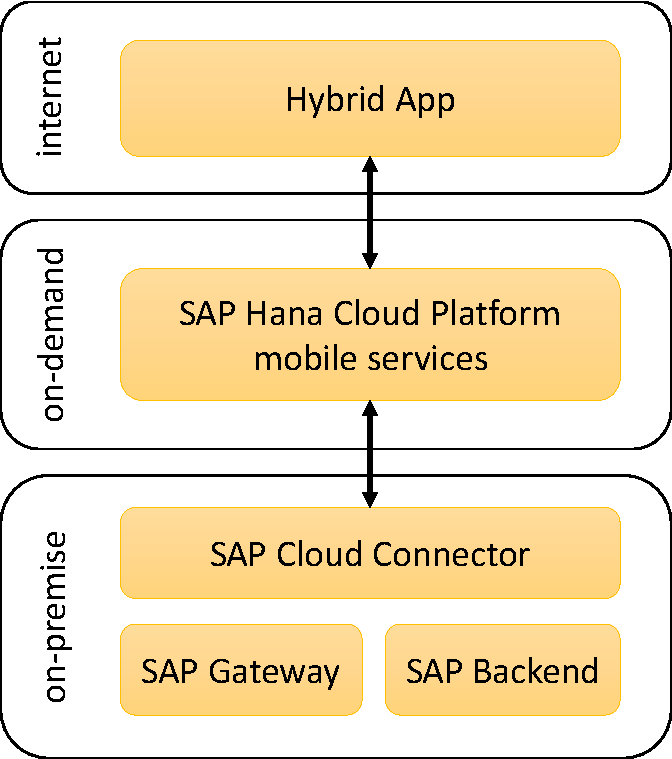
\includegraphics[width=.8\textwidth]{Architektur2} 
	\caption[App-Architektur]{App-Architektur nach \cite{openSAP2014_1}.}
	\label{fig:Architektur2}
\end{figure}

\subsection{Architektur}
\label{sec:app-architektur}
Wie im \autoref{sec:architekturen} beschrieben, gibt es viele Möglichkeiten eine UI5-App zu betreiben und zu veröffentlichen. Die Entscheidung richtet sich nach den benötigten Geräte- und Geschäftsfunktionen sowie der SAP-Integrationstiefe. 

In der ersten Version der Scrum-App sind weder Offline-Funktionen, noch native Gerätezugriffe gefordert. Einzig der Zugriff ohne Intranet-Verbindung erfordert besondere Beachtung. Die empfohlene Lösung ist die Weiterleitung des OData-Services nach außen über die Hana Cloud Platform, siehe \autoref{fig:Architektur2}. Der SAP Cloud Connector stellt die sichere Verbindung zwischen SAP-Backend vor Ort und der Cloud her. Vorteil: Das SAP-Backend des Kunden ist nach außen nicht sichtbar, die Firewall-Konfiguration muss nicht angepasst werden. App-Benutzer melden sich direkt an der Cloud-Plattform an, benötigen also keinen Intranet-Zugriff per VPN mehr.


%\subsection{Aufwandsschätzung}


\section{Testkonzept}
Das Testkonzept orientiert sich an IEEE\,829 \cite{IEEE829}, angepasst an die kleinere Projektgröße. Es ist als Dokument für alle Aktivitäten während des gesamten Projekts gültig. Darüber hinaus soll es als Vorlage für zukünftige App-Entwicklungen dienen. Ziel ist die Umsetzung des fundamentalen Testprozesses nach Spillner \cite{SpillnerRossnerWinterLinz2014}. In anderen Teilen der Arbeit behandelte Testwerkzeuge werden nicht beschrieben. Berücksichtigt werden folgende Dokumente:
\begin{itemize}
	\item Anforderungsspezifikation des Kunden, siehe \autoref{sec:app-spec}
	\item UI5 Development Conventions and Guidelines \cite{SAP2014_1}, insbesondere:
	\begin{itemize}
		\item JavaScript Coding Guidelines
		\item UI5 Control Development Guidelines
		\item Product Standards/Acceptance Criteria
		\item Git Guidelines
		\item File Names and Encoding	
	\end{itemize}
	\item SAP Gateway Best Practices (\cite[S.\ 561-563]{BoennenDreesFischerHeinzStrothmann2014})
	\item Projektvorgehen: Testgetrieben inkl. \ac{CI} (siehe \autoref{cha:Grundlagen})
\end{itemize}


\subsubsection{Testobjekte}
Der Architektur aus \autoref{sec:app-architektur} folgend, besteht die Anwendung aus zwei Hauptkomponenten. Beide sind Teil des Testkonzepts:
\begin{itemize}
	\item HTML5-Frontend (OpenUI5 1.26.8)
	\item SAP-Backend
	\begin{itemize}
		\item Funktionsbausteine (ECC 6.0, EHP 7, NW 7.4)
		\item OData-Service (SAP Gateway NW 7.4)
	\end{itemize}
\end{itemize}
Nicht einzeln getestet werden die JavaScript-Frameworks wie OpenUI5 und die verwendeten Test-Frameworks. Die Testbasis der entsprechenden Open-Source-Projekte ist mit diversen Unit- und Akzeptanztests sehr umfangreich. Eine projektinterne Test-Wiederholung bringt keinen Mehrwert.


\autsubsection{Steuerung und Planung}{Mattfeld}
Durch die kleine Teamgröße sind Entwickler gleichzeitig Tester (Test-Manager, Designer, Automatisierer, \dots).
Sie erarbeiten gemeinsam mit dem Kunden nach dem Prinzip des \ac{BDD} allgemein verständliche Anforderungen. Die Beschreibung der Fallbeispiele erfolgt im Schema von automatisierbaren \textit{Wenn-Dann}-Sätzen.

Fehlerkosten verdoppeln sich in jeder Entwicklungsphase. Der Kunde wird daher besonders stark in die Designphase einbezogen, um Kosten durch späte Änderungen zu vermeiden.

\subsubsection{Risiko und Kosten}
Insgesamt sind Fehlerkosten schwer abzuschätzen. Schadenshöhe und Wahrscheinlichkeit sind durch interne, ergänzende Verwendung der App überschaubar: Die Scrum-Aufgaben werden nur angeschaut oder im Status verändert. Nutzereingaben über den Client müssen allerdings immer als kritisch eingestuft werden. Gültigkeitsprüfungen in der App dienen nur der schnellen Rückmeldung an den User und Trafficvermeidung, nicht der Sicherheit. Das Backend ist daher ausführlich zu betrachten. 

Durch eine Fehlfunktion besteht eine Gefahr für laufende Projekte bei diversen Kunden. Daraus folgen direkte Schäden und Imageverlust. Fehlerkorrekturkosten werden durch TDD und CI eingegrenzt -- Regressionstests und Deployment sind automatisiert.

Testkosten sind ebenso schwierig vorauszusehen. Vor allem der geringe Reifegrad des Entwicklungsprozesses erschwert die Schätzung: Bisherige Erfahrungen sind durch den prototypischen Projekt-Charakter nicht vorhanden. Der Testplan kommt zum ersten Mal zum Einsatz. Allerdings wird die Testbarkeit und Modularität der Software durch testgetriebene Entwicklung sichergestellt. Zusätzlich ist die Testinfrastruktur von Anfang an vorhanden und erfüllt alle Anforderungen an Continuous Integration. Die Projektteilnehmer sind mit diesen Werkzeugen vertraut und beherrschen die Grundlagen des Testens nach ISTQB.

Die höchste Priorität haben die Tests des sicherheitskritischen Backends. In der App-Komponente decken die Akzeptanzkriterien Funktionalitäten mit hoher Nutzungshäufigkeit ab. Sie stehen im Mittelpunkt der Kundenwahrnehmung des Produktes und werden entsprechend wichtig eingestuft. 

Testaufwand: Eine vollständige Analyse der Aufwände ist nicht möglich und Erfahrungswerte sind noch nicht vorhanden. Diese Herausforderungen stellen ein großes Projektrisiko dar. Zumindest durch bekannte QM-Werkzeuge und hohe Automatisierung soll die Erfolgswahrscheinlichkeit erhöht werden. Den Testaufwand schätzen wir bei diesem Prototypen mit mindestens 50\,\% des Gesamtentwicklungsaufwands ein.

\subsubsection{Qualitätsziele und Testabedeckung}
Testendkriterium ist eine Anforderungsüberdeckung von 100\,\%. Ebenso müssen die sicherheitskritischen Äquivalenzklassentests des Backends zu 100\,\%. erfolgreich laufen. Testabbruchkriterien sind fehlgeschlagene Unit- und Akzeptanztests. Fehler der statischen Analyse führen ebenso zum Abbruch, Warnungen oder Schwankungen in den Komplexitäts-Metriken allerdings nicht.

Die nicht-funktionalen Anforderungen des UI5-Design-Guides können nur teilweise durch statische Analysen automatisiert überprüft werden. Gezielte Reviews während der Designphase und bei größeren Änderungen ergänzen die automatische Analyse. Die Performance der App wird im Rahmen der Systemtests überprüft. Die Akzeptanztests werden hierzu mit kurzen Timeouts angepasst.

\subsubsection{Konfigurationsverwaltung}
Die Konfigurationsverwaltung erfolgt per Git über die Plattform GitHub. Es gelten die UI5 Guidlines zu Git Commits: Es muss jederzeit nachvollziehbar sein, wer, wann, warum, welche Codezeilen geändert hat.

Eingecheckt wird nicht nur der Programmcode, sondern auch die Dokumentation, Tests und die CI-Toolchain. Das Prinzip \textit{Infrastructure as a Code} ist vollständig umgesetzt. Das bedeutet, die gesamte Build- und Deployment-Umgebung kann auf einem neuen System automatisch wiederhergestellt werden. 

Die Abhängigkeiten der Tool- und Framework-Versionen sind in Konfigurationsdateien hinterlegt und werden über die Paketmanager aufgelöst. Über Git werden Zwischenversionen der App gekennzeichnet oder in Branches ausgegliedert. Die Wiederherstellung eines bestimmten Entwicklungsschrittes inklusive Dokumentation, Buildumgebung und Tests ist stets gewährleistet. 

Das CI-System stellt die Gültigkeit der Konfigurationsverwaltung sicher. Jede Neuerung in der Versionskontrolle löst einen vollständigen Neuaufbau der Buildumgebung auf dem CI-Server anhand der Konfiguration aus.


\subsubsection{Fehlermanagement}
Ein Testprotokoll wird für jeden Build separat auf dem CI-Server vorgehalten. Das gesamte Projektteam hat Zugriff auf das Protokoll. Zusätzlich wird der Build-Status im Repository visualisiert. Das Team ist jederzeit über den Teststatus informiert.

Durch \ac{TDD} existiert theoretisch kein ungetesteter Code. Die QA-Pipeline wird in einem \textit{Private Build} auf dem Entwicklungsrechner komplett durchlaufen. Noch nicht implementierte Funktionalitäten bzw. die zugehörigen roten Tests werden auch nicht in die globale Versionsverwaltung eingecheckt. Neue Fehlerwirkungen werden vor allem während der höheren Teststufen wie Integrations-, System- und Akzeptanztests auftreten. Denkbar sind auch Inkompatibilitäten mit Browsern und Endgeräten oder Probleme mit dem CI-Prozess selbst.

 Da alle Projektartefakte in der Versionsverwaltung eingecheckt werden, ist auch das Fehlermanagement zentral für alle Projektteilnehmer. Das Schema einer Fehlermeldung ist festgelegt und beinhaltet eine eindeutige Fehlernummer, Entdecker, Erfassung und Problembeschreibung. Angaben zur zugehörigen Anforderung, Fehlerquelle und Reproduktion werden wenn möglich eingetragen. Über verschiedene Labels werden für dieses Projekt individuell gesetzt: Fehlerklasse (Bug, Enhancement, Documentation), Priorität (open, wontfix) und Status (new, open, approved, invalid, question, duplicate, works, fixed).

Testfälle und Korrekturen werden über einen Fork eingebracht. Beides kann per Kommentarfunktion diskutiert werden. Ist der Fehler durch einen Testfall nachgewiesen und die Code-Korrektur akzeptiert, schließt ein Kommentar im Commit automatisch das Issue Ticket.

%\subsection{Design und Analyse}
%Testbasis prüfen (Anforderungen), Testbarkeit prüfen, Logische Testfälle

\subsection{Durchführung}
\label{sec:tests}
Die Testfälle unterteilen sich in verschiedene Teststufen:
\begin{itemize}
	\item Komponententests der Funktionsbausteine
	\item Integrationstests zwischen Backend und Gateway
	\item Isolierter Akzeptanztests der App mit Mockserver
	\item Systemtest mit App und Gateway
\end{itemize}

\subsubsection{Akzeptanztest-Szenario 1: Kundenübersicht}

\textbf{Given} I start the app\\
\textbf{When} I look at the screen\\
\textbf{Then} I should see the customer list\\
\textit{and} the customer list should have entries\\

\subsubsection{Akzeptanztest-Szenario 2: Projektübersicht}

\textbf{Given} I start the app\\
\textbf{When} I press on customer 1\\
\textbf{Then} I should be taken to customer 1\\
\textit{and} I should see the project list of customer 1\\
\textit{and} the project list should have entries\\



\subsubsection{Äquivalenzklassentest}
Um alle möglichen Eingabewerte für einen Funktionsbaustein zu ermitteln, werden Äquivalenzklassen für die jeweiligen Eingabeparameter gebildet, siehe \autoref{tab:aquivalenzklassen-FubaProjekte}. Hierbei ist darauf zu achten, dass für jeden Parameter auch negative Werte getestet werden. Da die Anzahl der Testfälle bei einfacher Multiplikation der möglichen Kombinationen schnell zu einer erheblichen Anzahl ansteigt, werden gültige Äquivalenzklassen in den Testfällen kombiniert. Ungültige Äquivalenzklassen dürfen wiederum nur mit gültigen Äquivalenzklassen kombiniert werden, sodass für jede ungültige Äquivalenzklasse ein eigener Testfall erstellt wird \cite[S.\ 110-115]{Spillner2010}. Die daraus entstandenen Testfälle sind in \autoref{tab:test-read-projektet} zu sehen. Damit wird eine Äquivalenzklassenüberdeckung von 100\,\% für den zu testenden Funktionsbaustein erreicht.

\begin{table}[h]
	\centering
\begin{tabular}{cccc}
	\toprule Äquivalenzklasse & Parameter & Eingabewert & ÄK gültig?\\
	\midrule ÄK1 & Kunde  & ''TKMI''  & Ja\\ 
			ÄK2 & Kunde & ''tkmi'' & Nein\\
			ÄK3 & Kunde & - & Nein\\
			\midrule
			ÄK4 & Projekt & ''TM-SCRUM'' & Ja\\
			ÄK5 & Projekt & ''tm-scrum'' & Nein\\
			ÄK6 & Projekt & - & Ja\\
			\midrule
			ÄK7 & Substring & ''TM-SCRUM'' & Ja\\
			ÄK8 & Substring & ''tm-scrum'' & Ja\\
			ÄK9 & Substring & ''asdf'' & Nein\\
			ÄK10 & Substring & - & Ja\\
			\midrule
			ÄK11 & Projekt und Substring & nicht leer & Nein\\
	\bottomrule 
\end{tabular} 
\caption{Äquivalenzklassen für den Funktionsbaustein Z\_SCRUMUI5\_READ\_PROJEKTE}
\label{tab:aquivalenzklassen-FubaProjekte}
\end{table} 

\begin{table}[h]
	\centering
\begin{tabular}{cccccc}
	\toprule Testfall & getestete ÄK & Kunde 	& Projekt 		& Substring 	&  Ergebnis \\ 
	\midrule     1 	 &  1,6,10 		& ''TKMI'' 	& - 			& - 			&  Anzeige erfolgt\\ 
			 2 	 & 4			& ''TKMI'' 	&''TM-SCRUM'' & - 			& Anzeige erfolgt\\ 
			 3	 &  7			& ''TKMI'' 	& - 			& ''TM-SCRUM'' & Anzeige erfolgt\\ 
			 4	 &  8			& ''TKMI'' 	& - 			& ''tm-scrum''	& Anzeige erfolgt\\ 
			5 	 &  2			& ''tkmi'' 	& - 			& - 			& Keine Anzeige\\ 
			6 	 &  3			& - 		& - 			& - 			& Keine Anzeige\\ 
			7 	 &  5			& ''TKMI'' 	& ''tm-scrum''	& - 			& Keine Anzeige\\ 
			8 	 &  9			& ''TKMI'' 	& - 			& ''asdf'' 		& Keine Anzeige\\ 
			 9 	 & 11			& ''TKMI'' 	& ''TM-SCRUM''	& 'TM-SCRUM''		& Keine Anzeige\\ 
	\bottomrule 
\end{tabular} 
\caption{Ermittelte Testfälle für den Funktionsbaustein Z\_SCRUMUI5\_READ\_PROJEKTE}
\label{tab:test-read-projektet}
\end{table} 

%Äquivalenzklassen-Überdeckung = (Anzahl getesteter ÄK / Gesamtanzahl ÄK) x 100\%

\subsubsection{Testfälle OData-Service}
Die relevanten Testfälle (siehe \autoref{tab:testfälle-OData}) für den OData-Service werden durch die verwendeten OData-Funktionen bestimmt. Dabei ist zwischen den allgemeinen Testfällen für den kompletten OData-Service, sowie den Funktionen die für jede Entität einzeln getestet werden zu unterscheiden.

\begin{table}[h]
	\centering
\begin{tabular}{ccccc}
	\toprule Testfall & OData-Funktion  \\
	\midrule 	
	Allgemeine Testfälle: & \\
	\midrule
	TF1 & JSON-Format \\
	 	    	TF2 & Servicedokument \\
			TF3 & \$metadata\\
	\midrule
	Testfälle je Entität: & \\
	\midrule		
			TF4 & \$expand\\
			TF5 & Navigation\\
			TF6 & Navigation mit \$links\\
			TF7 & \$count \\
			TF8 & \$ordberby\\
			TF9 & \$skip\\
			TF10 & \$top\\
			TF11 & GetEntititySet\\
			TF12 & GetEntitity\\
			TF13 & \$filter\\
	\bottomrule 
\end{tabular} 
\caption{Testfälle - OData-Service}
\label{tab:testfälle-OData}
\end{table} 

\chapter{Implementierung}
\label{cha:Implementierung}
\autsection{Backend}{Azimi}
\subsection{Werkzeuge}

Für die verschiedenen Abschnitte im Entwicklungsprozess eines Gateway-Services stellt SAP folgende Werkzeuge zur Verfügung.

\subsubsection{OData Modeler}
\label{sec:OData-Modeler}
Das grafische Werkzeug zur OData-Service-Modellierung ist als Eclipse-Plugin in den \textit{SAP Mobile Platform Tools} enthalten. Entitäten werden inklusive (Navigations-)Eigenschaften und Abhängigkeiten definiert, siehe \autoref{fig:OData-Modeler}.

Die Service-Metadaten werden als XML-Datei exportiert und vom UI5-Mock-Server genauso importiert wie vom Service Builder des SAP Gateway. Eine direkte Verbindung zum SAP-System und Import/Export bestehender Services ist ebenso möglich. Ab der Service-Definition laufen Front- und Backend-Entwicklung unabhängig voneinander.

\begin{figure}[h]
	\centering
	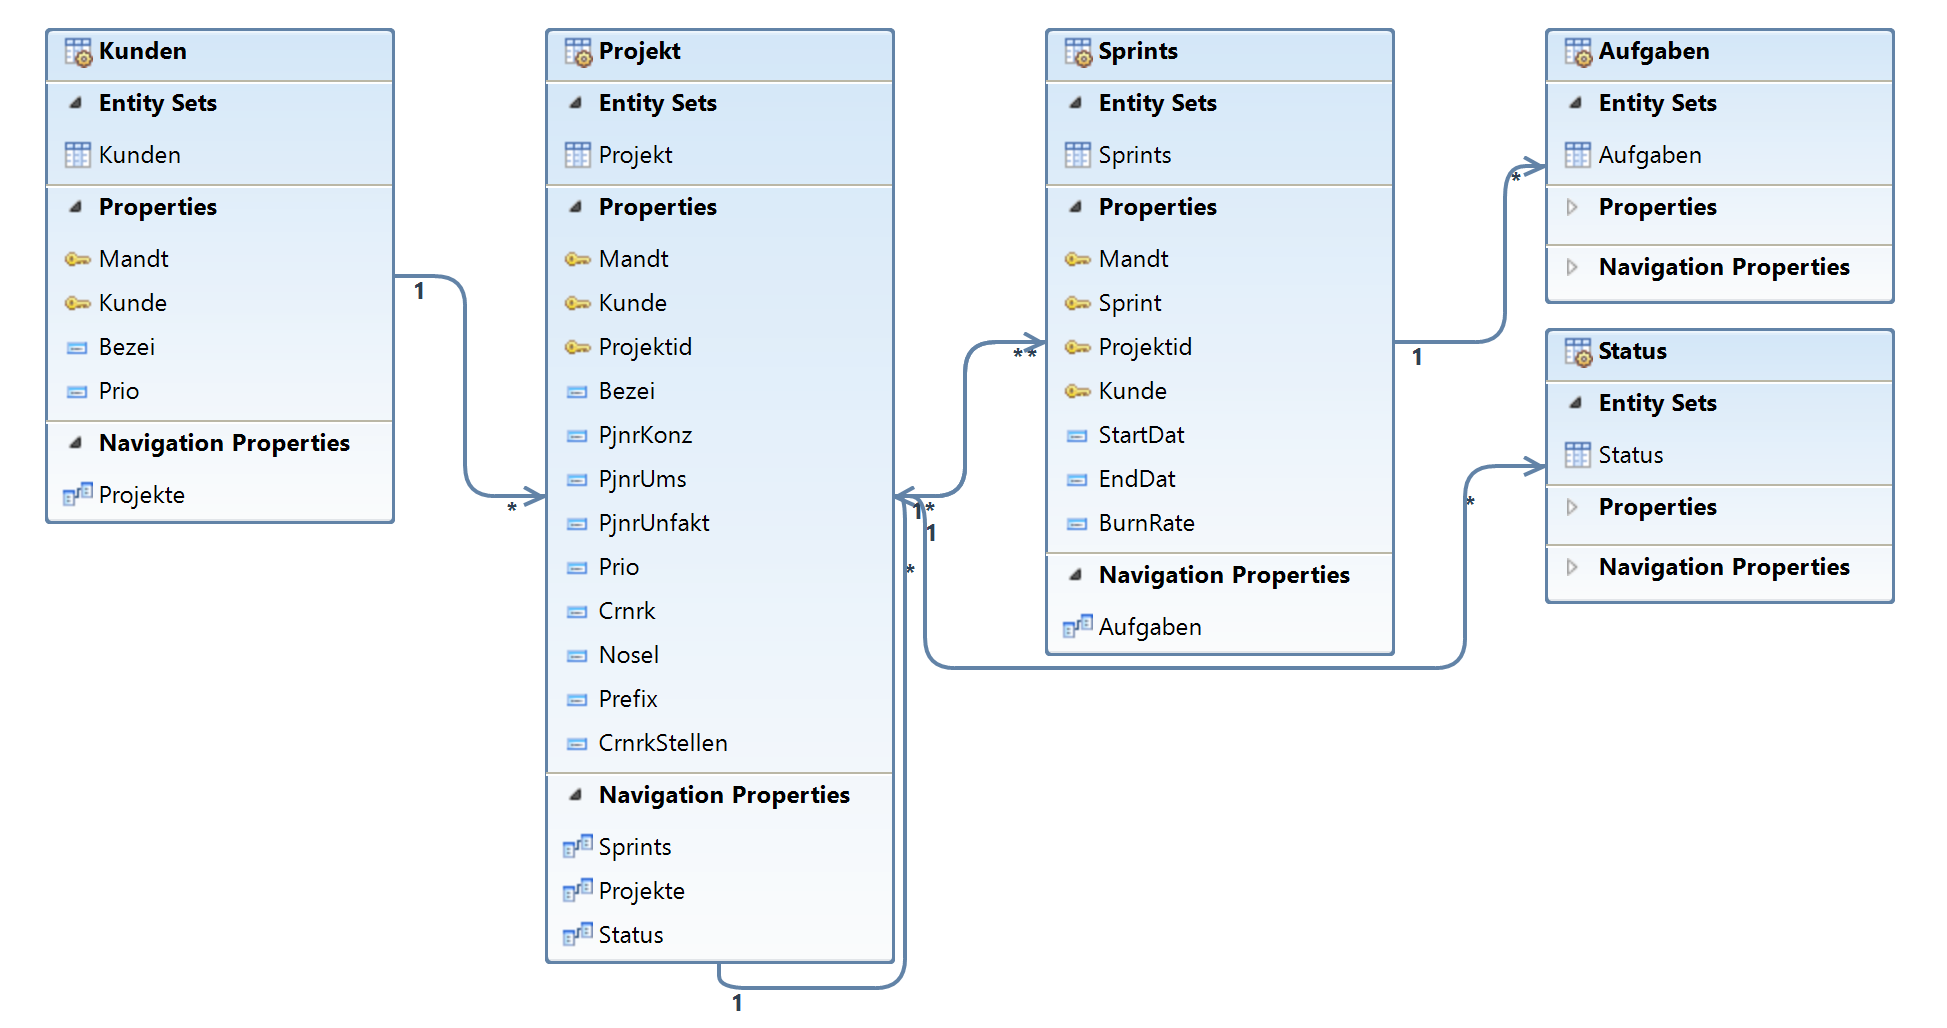
\includegraphics[width=1.25\textwidth]{odata-modeler} 
	\caption[OData Modeler]{OData Modeler.}
	\label{fig:OData-Modeler}
\end{figure}

\subsubsection{SAP Gateway Service Builder}
Das zentrale Werkzeug zur Erstellung von OData-Services ist der SAP Gateway Service Builder (Transaktion \emph{SEGW}). Der Service Builder enthält alle Funktionalitäten, die für die Serviceentwicklung benötigt werden \cite[S.\ 187-189]{BoennenDreesFischerHeinzStrothmann2014}. 


\subsubsection{Gateway-Client}
\label{sec:gateway-client}
Zum Testen des OData-Services wird der sogenannte Gateway-Client (Transaktion \emph{/IWFND/GW\_CLIENT}) verwendet. Mit ihm lassen sich alle Funktionalitäten des zuvor erstellten OData-Services testen. Testfälle lassen sich definieren und in Testgruppen zusammenzufassen, um sie später erneut auszuführen \cite[S.\ 190-192]{BoennenDreesFischerHeinzStrothmann2014}.


\subsubsection{Fehlerprotokoll}
Zur Fehlerbehandlung gibt es das Fehlerprotokoll unter der Transaktion \emph{/IWFND/ERROR\_LOG}. Hier laufen alle Fehler auf, die beim Aufruf von Gateway-Services auftreten. Bei Bedarf ist es dank Integration des Gateway Clients möglich, eine fehlerhafte Abfrage erneut auszuführen \cite[S.\ 192-193]{BoennenDreesFischerHeinzStrothmann2014}.
%193 - Syslog und Anwendungsprotokoll?

\subsubsection{Services aktivieren und verwalten}
In der Transaktion \emph{/IWFND/MAINT\_SERVICE} werden neue Services registriert und aktiviert. Ausgewählte Services lassen sich im Browser oder Gateway-Client testen und das dazugehörige Fehlerprotokoll wird, wenn nötig, geöffnet \cite[S.\ 571-573]{BoennenDreesFischerHeinzStrothmann2014}.


\subsection{Funktionsbausteine}
Für den Zugriff auf Daten aus dem SAP-Backend werden in der zentralen Aufgabenverwaltung derzeit Funktionsbausteine verwendet. Diese werden remotefähig gemacht, um über die \ac{RFC}-Schnittstelle aufrufbar zu sein. Für die Abfrage der Daten werden die \ac{RFC}-Funktionsbausteine vom OData-Service mit entsprechenden Parametern aufgerufen. Die RFC-Funktionsbausteine kommen dann beim Lesen der Kunden-, Projekt-, Sprint-  und Aufgabendaten sowie der möglichen Aufgabenstatus der einzelnen Projekte zum Einsatz. 

\begin{listing}[H]
	\inputminted{abap}{src/fubaprojekte.abap}
	\caption{Z\_SCRUMUI5\_READ\_PROJEKTE}
	\label{lst:Quellcode-ReadProjekte}
\end{listing}

\subsubsection{Entwicklung}
In allen Funktionsbausteinen werden Importparameter definiert, die vom OData-Service übergeben werden können. Dieses sind in der Regel die Primärschlüssel der Datenbanktabellen, auf die durch einen Funktionsbaustein zugegriffen wird, um eindeutige Datensätze auslesen zu können. Zusätzlich wird ein Parameter zur Filterung nach Teil-Strings definiert. Die ausgelesenen Daten werden über eine Tabelle, mit der Struktur der ursprünglichen Datenbanktabelle, zurückgegeben.

Im Listing \ref{lst:Quellcode-ReadProjekte} wird der Funktionsbaustein zum Auslesen der Projektdaten dargestellt. Es gibt drei mögliche Szenarien zum Aufruf des Bausteins mit den jeweils nötigen Übergabeparametern:

\begin{enumerate}
	\item Alle Projekte eines Kunden (KundenID)
	\item Ein bestimmtes Projekt des Kunden (KundenID, ProjektID)
	\item Projekte des Kunden die Teil-String enthalten (KundenID, ProjektID)
\end{enumerate}
In den ersten beiden Szenarien werden einfache Select-Statements auf die Datenbanktabellen ausgeführt um auf die Daten zuzugreifen. Da mit dem SQL Like Operator im Open SQL die Nichtbeachtung von Groß- und Kleinschreibung nicht möglich ist, wird im letzten Szenario, nach dem Select-Statement, durch alle zurückgegebenen Datensätze gelaufen und überprüft ob der übergebene Teil-String in der Bezeichnung des Projektes vorhanden ist. Hierbei ist es dann egal, ob die Groß- und Kleinschreibung des Datenbankeintrages identisch mit der des Teil-Strings ist.


\subsubsection{Testen}
Zum Testen von neuen Funktionsbausteinen gibt es in der ABAP Workbench die Funktion den jeweiligen Funktionsbaustein auszuführen und zu testen. Dazu wählt man in der Drucktastenleiste \textit{Testen/Ausführen (F8)}. Man gelangt auf das Bild \textit{Funktionsbaustein testen: Eingabebild}. Hier werden alle Import-Parameter des Funktionsbausteins angezeigt. Nach Eingabe der Parameter kann der Funktionsbaustein mit \textit{Ausführen (F8)} gestartet werden. Der Funktionsbaustein wird mit den eingetragenen Importparametern ausgeführt und vorhandene Exportparameter oder Tabellen werden nach Ausführung angezeigt. 


\begin{figure}[h]
	\centering
	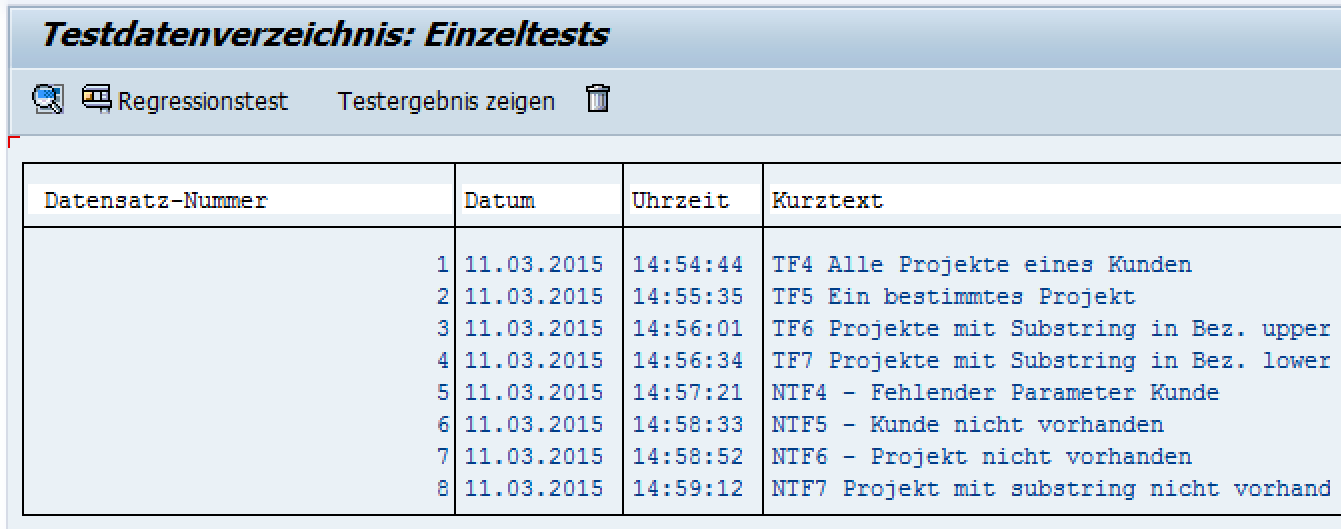
\includegraphics[width=.95\textwidth]{Testdatenverzeichnis} 
	\caption[Funktionsbaustein -- Testdatenverzeichnis]{Funktionsbaustein -- Testdatenverzeichnis.}
	\label{fig:Testdatenverzeichnis}
\end{figure}

\begin{figure}[h]
	\centering
	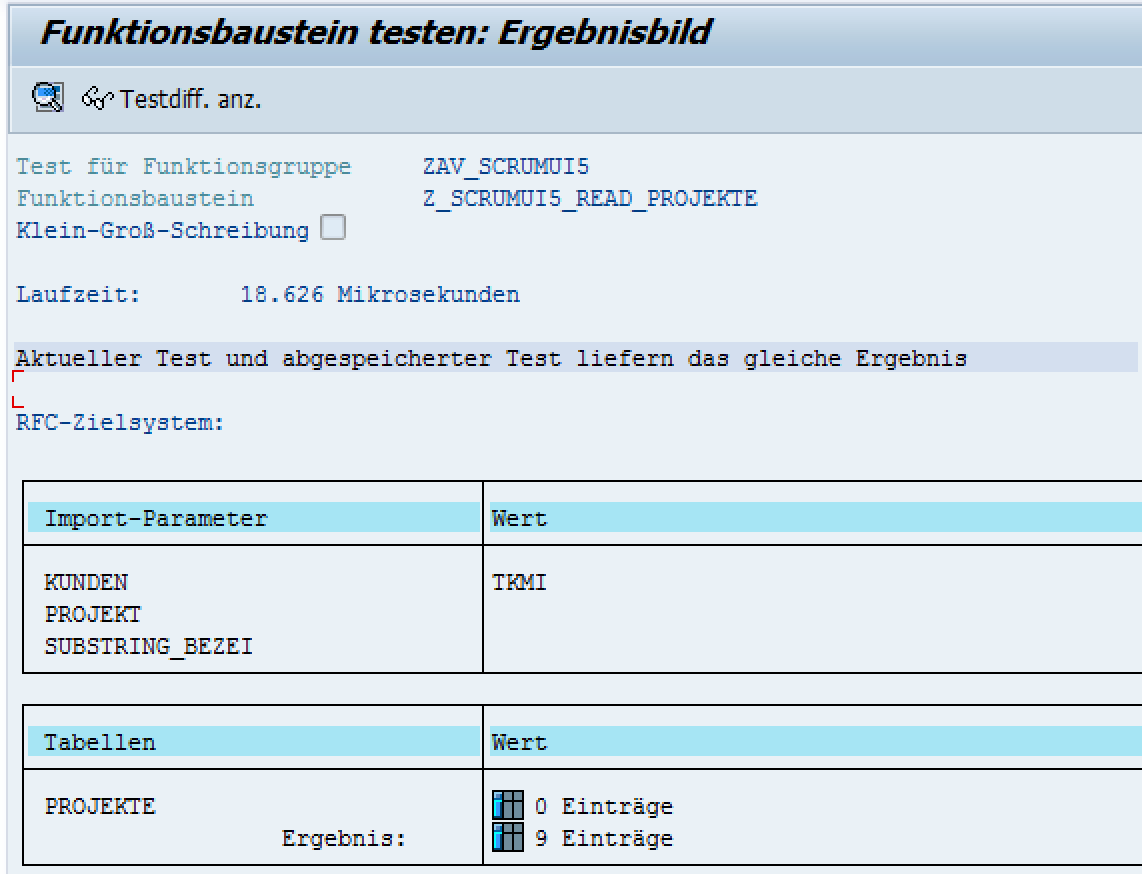
\includegraphics[width=.95\textwidth]{Regressionstest} 
	\caption[Funktionsbaustein -- Regressionstest]{Funktionsbaustein -- Regressionstest.}
	\label{fig:Regressionstest}
\end{figure}

Es ist möglich Testfälle im Testdatenverzeichnis zu speichern. Das Testdatenverzeichnis erreicht man über den ersten Eingabebildschirm. Alle gespeicherten Testfälle werden mit Erstelldatum und Kurztext wie in \autoref{fig:Testdatenverzeichnis} angezeigt und lassen sich hierüber erneut aufrufen. Bei Ausführung eines  Regressionstest wird im Ergebnis angezeigt ob sich das Ergebnis seit dem Speichern des Testes verändert hat, siehe \autoref{fig:Regressionstest}. Falls eine Differenz zum gespeichertem Ergebnis vorhanden ist, lässt sich diese anzeigen.\\ 



\subsection{OData-Service}
Für die Erstellung eines OData-Services im SAP Gateway gibt es generell unterschiedliche Wege: Zum einen gibt es die Serviceentwicklung mit \ac{ABAP}, welches flexiblere und effizientere Services ermöglicht. Diese erfordert allerdings spezielles \ac{ABAP}-Know-how. 

Alternativen dazu sind die Servicegenerierung durch den \ac{RFC}/\ac{BOR}-Generator, die Redefinition oder die Model Composition von bereits vorhandenen Gateway-Services. Die Servicegenerierung führt zu schnelleren Ergebnissen, ist durch eingeschränkte Rechte allerdings oft nicht weiter anpassbar.

Im Normalfall rechtfertigen die Vorteile durch die klassische ABAP-Service-Entwicklung den höheren Aufwand. Die Möglichkeit der Servicegenerierung wird interessant, sobald es geeignete Datenquellen für die automatische Generierung gibt \cite[S.\ 181]{BoennenDreesFischerHeinzStrothmann2014}.

Generell wird ein inkrementeller Serviceerstellungsprozess empfohlen, in dem der Service \bzw Teile davon direkt ausgeführt und getestet werden. Danach kann der Service so lange verändert werden, bis schließlich alle Anforderungen erfüllt werden \cite[S.\ 184]{BoennenDreesFischerHeinzStrothmann2014}.


\subsubsection{Entwicklung}
Die Entwicklung eines Gateway-Services lässt sich in drei Phasen einteilen:

\begin{quote}
	\begin{enumerate}
		\item Definition des Datenmodells
		\item Serviceimplementierung
		\item Serviceverwaltung
	\end{enumerate}
\end{quote}
%Definition des Datenmodells mit dem OData Modeler auf Basis der vorhandenen Struktur?
Zur \textit{Definition des Datenmodells} im SAP Gateway Service Builder gibt es unterschiedliche Varianten. 
Dazu zählen unter anderem die manuelle Deklaration des Datenmodells im Service Builder. Hierbei werden die Entitätstypen, Assoziationen und Assoziationsmengen manuell angelegt.

Alternativ kann ein bereits vorhandenes Datenmodell importiert werden, welches \zB mit dem OData Modeler erstellt wurde. Falls eine bereits vorhandene Datenstruktur aus einem SAP-System genutzt werden soll, können die Entitätstypen über einen DDIC-Import oder über den Import von \ac{RFC}/\ac{BOR}-Schnittstellen generiert werden \cite[S.\ 194-195]{BoennenDreesFischerHeinzStrothmann2014}.

\begin{figure}[h]
	\centering
	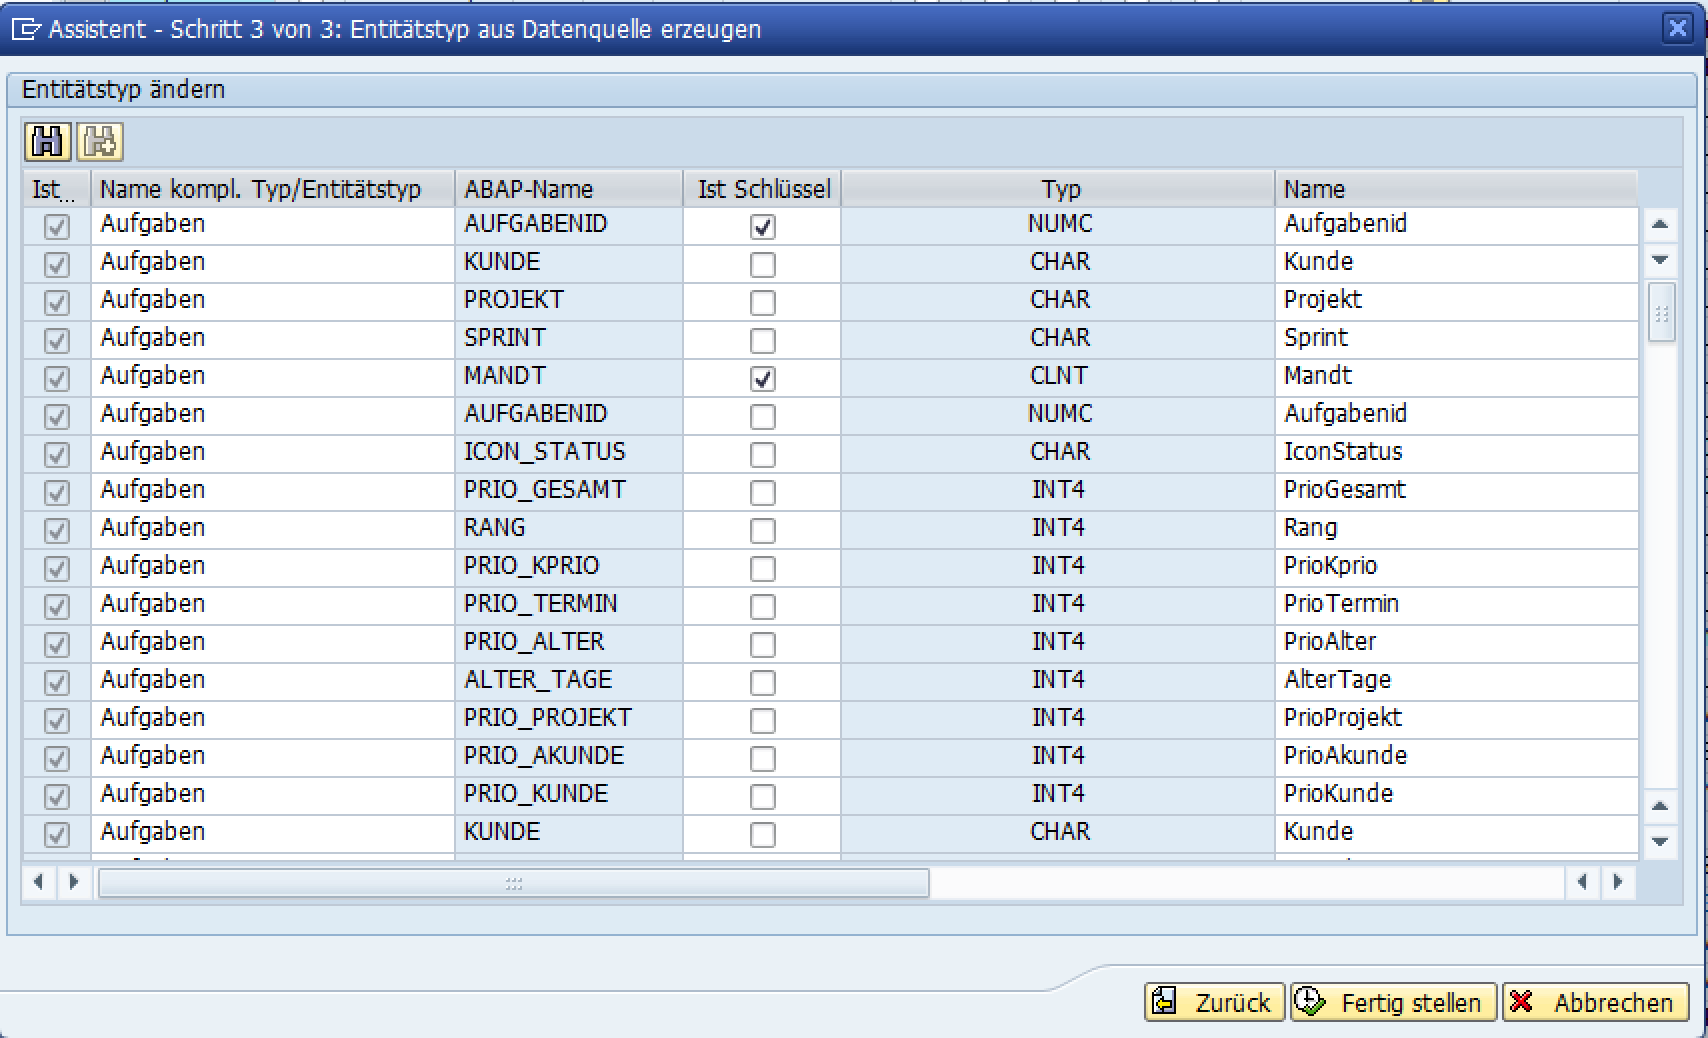
\includegraphics[width=.95\textwidth]{ImportRFC} 
	\caption[Import-RFC-Funktionsbaustein]{Import-RFC-Funktionsbaustein \cite[S.\ 45]{BoennenDreesFischerHeinzStrothmann2014}.}
	\label{fig:ImportRFC}
\end{figure}

In unserem Fall kommt der Import über RFC-Funktionsbausteine wie in \autoref{fig:ImportRFC} zum Einsatz, da diese auch für den Zugriff auf Daten aus dem SAP-Backend genutzt werden. Während des Imports des RFC-Funktionsbausteins müssen die Primärschlüssel der Entitätstypen festgelegt werden.

Unter den Eigenschaften der Entitätstypen lassen sich die einzelnen Attribute der Entitätstypen anzeigen und deren Eigenschaften ändern. So wird etwa definiert, ob ein bestimmtes Attribut sortier- oder filterbar ist. Diese Eigenschaften werden im Service-Metadatendokument hinterlegt. Diese haben allerdings nur einen informativen Charakter: Es erfolgt keine weitere Überprüfung durch das Gateway-Framework. So können Attribute sortiert werden, für die keine Sortier-Eigenschaft gesetzt wurde. 


Als nächstes müssen die Entitätsmengen definiert werden, die im Regelfall in einer 1:1-Beziehung zu den Entitätstypen stehen. Der spätere Zugriff über den OData-Service läuft immer über die Entitätsmengen und nicht über die Entitätstypen. Auch hier gibt es einige Attribute zu pflegen, \zB, ob ein Eintrag eines Entitätstypen angelegt, aktualisiert oder gelöscht werden darf, oder ein Filter für die Abfrage der Entitätsmenge zwingend erforderlich ist. Wie auch die Annotationen der Entitätstypen sind auch diese nicht zwingend bindend und erforderlich, sollten jedoch passend zum tatsächlichen Funktionsumfang des OData-Services gepflegt werden. So ist es für Service-Konsumenten einfacher herauszufinden, welchen Funktionsumfang der OData-Service unterstützt \cite[S.\ 237-240]{BoennenDreesFischerHeinzStrothmann2014}.


Anschließend wird der Service im SAP-System registriert. Hier werden die Laufzeitobjekte, die für den Gateway-Service benötigt werden, generiert \cite[S.\ 198]{BoennenDreesFischerHeinzStrothmann2014}.
Danach geht es an die \textit{Serviceimplementierung}. Hier gibt es die Auswahl zwischen der Implementierung durch ABAP-Programmierung  oder das Mappen von \ac{RFC}/\ac{BOR}-Schnittstellen \cite[S.\ 201-202]{BoennenDreesFischerHeinzStrothmann2014}.

\piccaption[RFC-Mapping]{RFC-Mapping\label{fig:MappingRFC}.}
\parpic{
	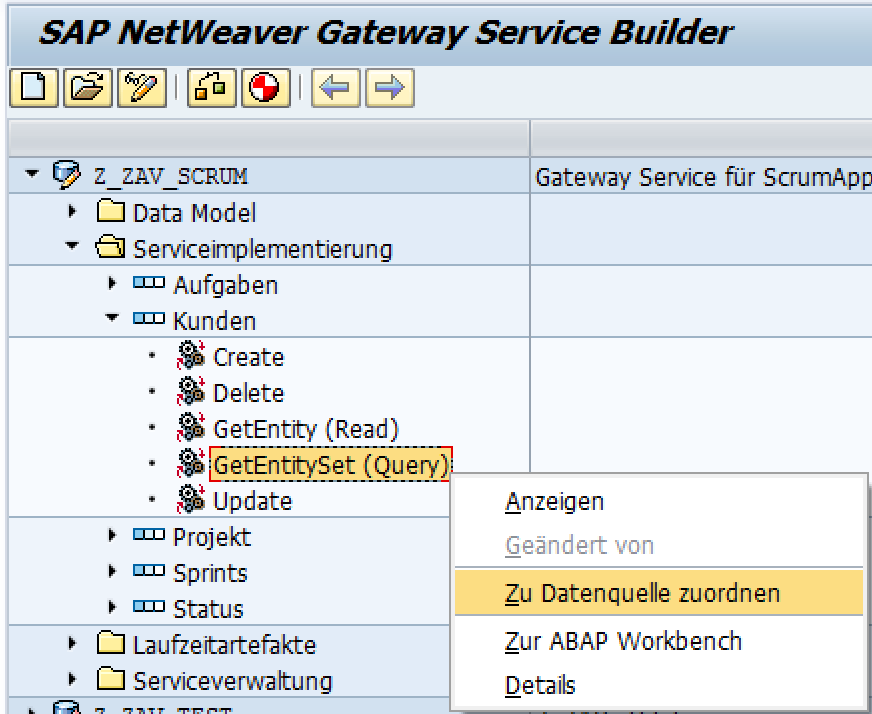
\includegraphics[width=.5\textwidth]{MappingRFC}
}

Um die Attribute einer En\-ti\-täts\-men\-ge mit einem RFC-Funk\-tions\-bau\-stein zu mappen, wählt man \emph{Zu Da\-ten\-quel\-le zuordnen} für den gewünschten Vorgang einer En\-ti\-täts\-men\-ge, hier: GetEntitySet der En\-ti\-täts\-men\-ge Kunden, siehe \autoref{fig:MappingRFC}.

Nach Angabe des Funk\-tions\-bau\-steins können die Attribute der Quelle zugeordnet werden. 

Dies funktioniert manuell oder über den Button \emph{Zuordnung vorschlagen} wie in \autoref{fig:MappingRFC2}. Zu diesem Zeitpunkt ist lediglich das Abrufen von Daten ohne zusätzliche Funktionen möglich. Um die Filterfunktionen des OData-Services nutzen zu können, müssen die Import-Parameter der Funktionsbausteine zugeordnet werden.

Dafür wird eine neue Zeile mit der Entitätsmenge des Importparameters hinzugefügt -- In diesem Fall \textit{Kunde}. Dieser wird dem Import-Parameter aus der Datenquelle zugeordnet. Jetzt kann nach bestimmten Kunden gefiltert werden.
So lassen sich Services mit Grundfunktionen relativ einfach durch die Servicegenerierung erstellen. Sobald Funktionen wie das Filtern nach Teil-Strings benötigt werden, ist eine Zusatzimplementierung durch ABAP-Programmierung notwendig.



\begin{figure}[h]
	\centering
	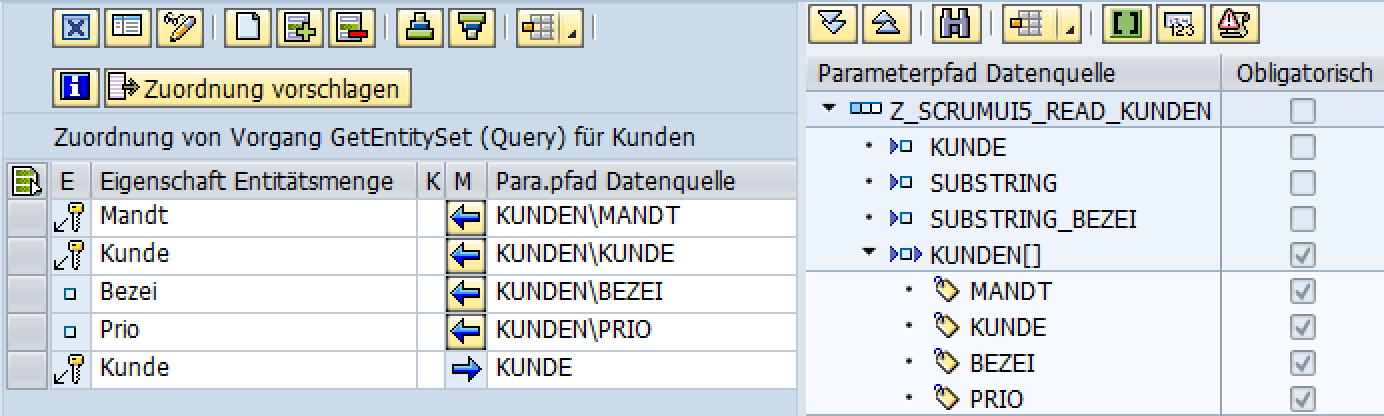
\includegraphics[width=.95\textwidth]{MappingRFC2} 
	\caption[RFC-Mapping -- Zuordnung der Attribute]{RFC-Mapping -- Zuordnung der Attribute.}
	\label{fig:MappingRFC2}
\end{figure}

Falls der Service durch ABAP-Programmierung erstellt werden soll, müssen die Methoden für den Vorgang in der ABAP-Workbench redefiniert werden. Die bei der Servicegenerierung automatisch erstellte Methode wird hier selbst implementiert. Alle Parameter, die vom OData-Service an das Gateway gesendet werden, müssen berücksichtigt und die entsprechenden Funktionen implementiert werden.

In \autoref{tab:ODataQueryOptions} gibt es eine kurze Übersicht, der vom SAP Gateway unterstützen OData-Query-Optionen, wovon einige eine zusätzliche Implementierung benötigen.

\begin{table}[h]
	\centering
	\begin{tabular}{cc}
		\toprule OData-Query-Optionen & Zusätzliche Implementierung notwendig \\ 
		\midrule \$select & Nein\\
		\$count & Nein\\
		\$expand & Nein\\
		\$format & Nein\\
		Read \$links & Nein\\
		\$value & Nein\\
		\$orderby & Ja\\
		\$top & Ja\\
		\$skip & Ja\\
		\$filter & Ja\\
		\$inlinecount & Ja\\
		\$skiptoken & Ja\\
		\bottomrule 
	\end{tabular} 
	\caption{Unterstützte OData-Query-Optionen im SAP Gateway aus \cite{SAP2015_3}}
	\label{tab:ODataQueryOptions}
\end{table} 



\begin{listing}[H]
	\inputminted{abap}{src/kundengetentityset.abap}
	\caption{KUNDEN\_GET\_ENTITYSET}
	\label{lst:Quellcode}
\end{listing}

In Listing \ref{lst:Quellcode} wird, falls in der Abfrage angegeben, ein Teil-String der Kundenbezeichnung in einer Variablen gespeichert. Diese wird anschließend an den Funktionsbaustein übergeben. Je nach Abfrage werden alle Kunden oder nur Kunden mit Teil-String im Namen zurückgegeben. Zum Abschluss werden die zurück erhaltenen Daten in die Tabelle \emph{ET\_ENTITYSET} geschrieben und an den OData-Service übergeben.

Nach Implementierung des Services muss dieser noch über die \textit{Serviceverwaltung} beim Gateway-Server registriert und aktiviert werden. Anschließend kann der OData-Service getestet werden.
Sind voneinander abhängige Entitätstypen im Service vorhanden, werden die Relationen mit den entsprechenden Kardinalitäten zwischen den Entitätstypen in den Assoziationen wie in \autoref{fig:Assoziationen} definiert. Die zuvor erstellten Assoziationen werden anschließend den Entitätstypen als Navigationseigenschaften zugewiesen, siehe \autoref{fig:Navigationseigenschaften}.

\begin{figure}[h]
	\centering
	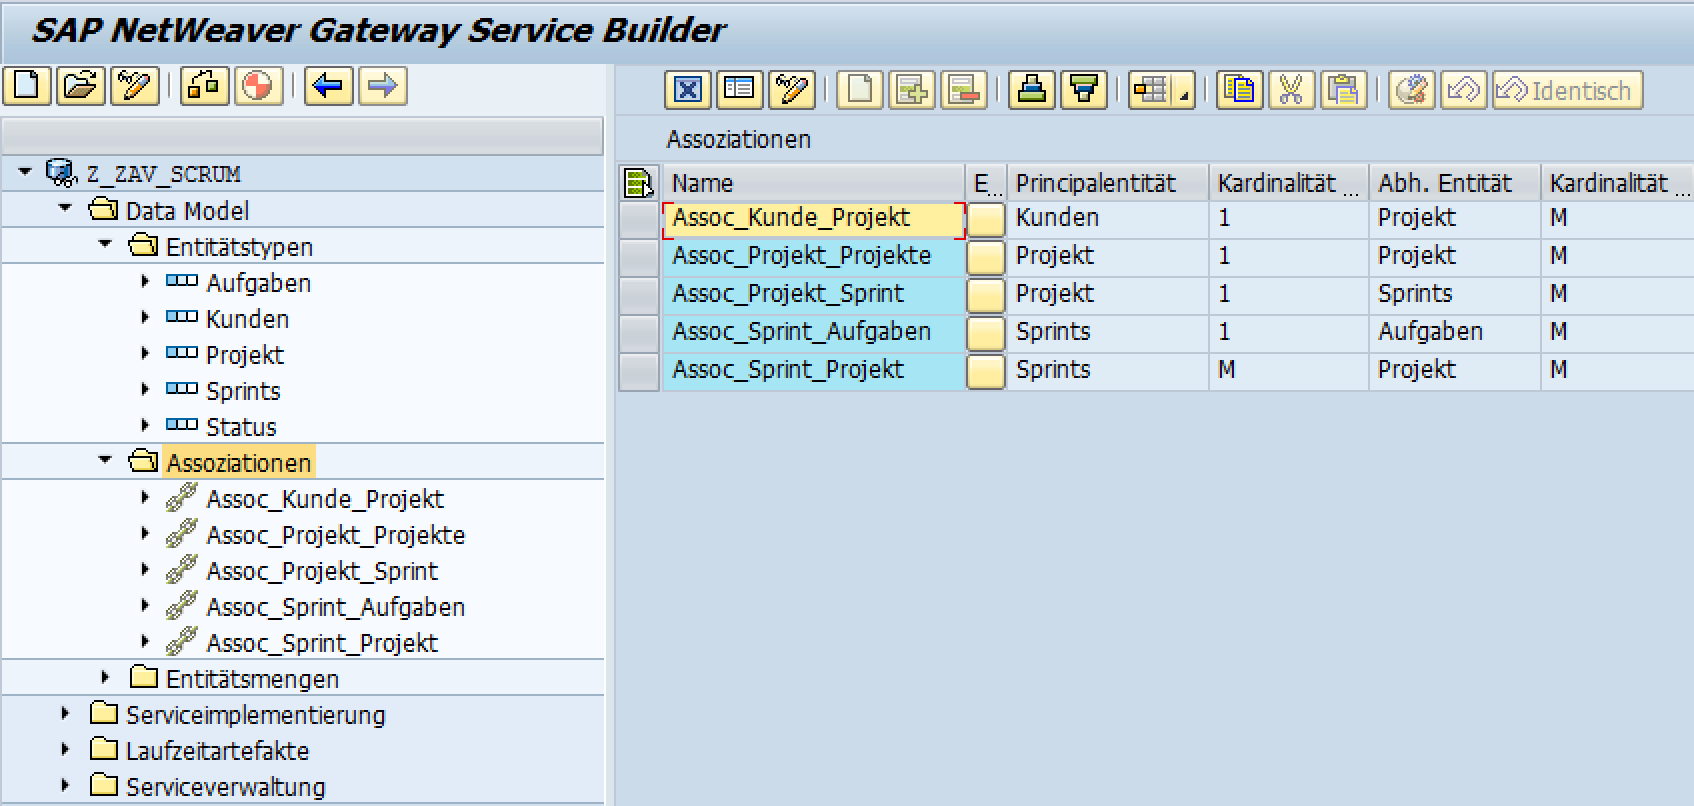
\includegraphics[width=.95\textwidth]{Assoziationen} 
	\caption[Entitätstypen -- Assoziationen]{Assoziationen zwischen den Entitätstypen.}
	\label{fig:Assoziationen}
\end{figure}


\begin{figure}[h]
	\centering
	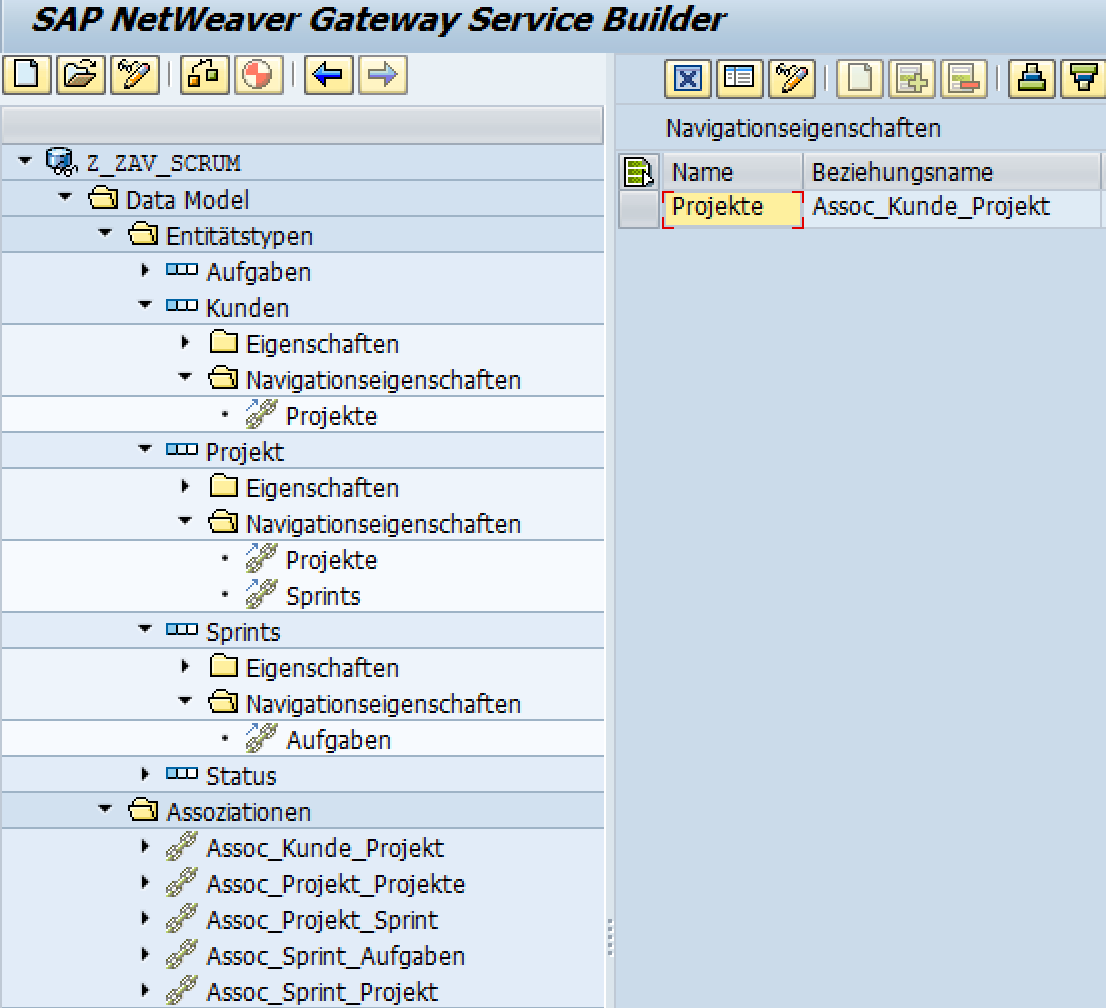
\includegraphics[width=.75\textwidth]{Navigationseigenschaften} 
	\caption[Entitätstypen -- Navigationseigenschaften]{Navigationseigenschaften zwischen den Entitätstypen.}
	\label{fig:Navigationseigenschaften}
\end{figure}


\subsubsection{Testen}

\begin{figure}
	\centering
	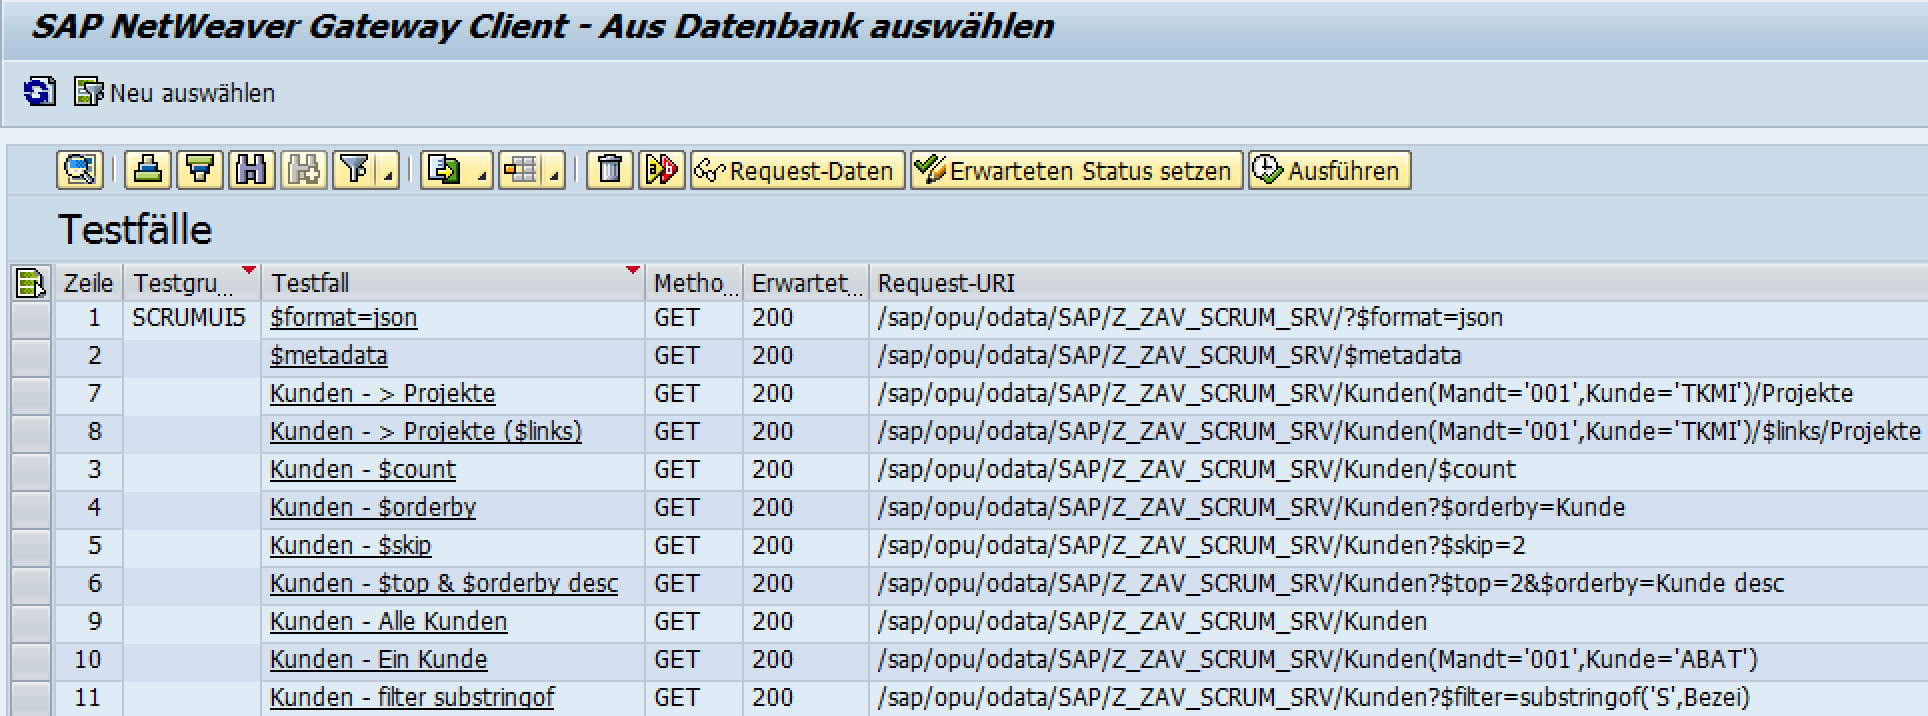
\includegraphics[width=.95\textwidth]{Testfalldatenbankodata} 
	\caption[OData-Testfalldatenbank]{OData-Testfalldatenbank.}
	\label{fig:Testfalldatenbankodata}
\end{figure}


\begin{figure}
	\centering
	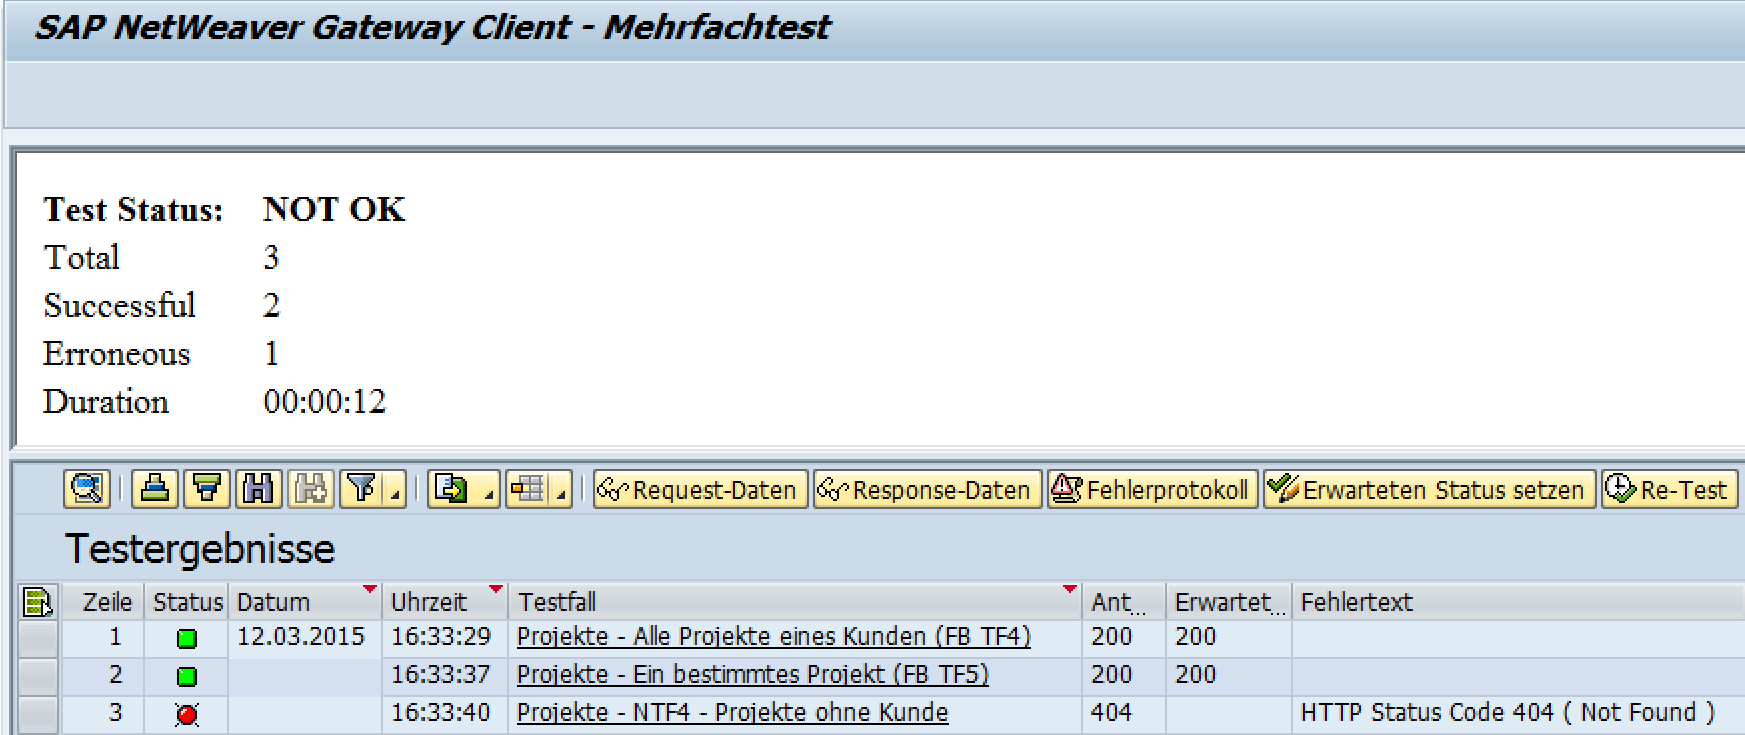
\includegraphics[width=.95\textwidth]{Mehrfachtest} 
	\caption[OData-Mehrfachtest]{OData-Mehrfachtest.}
	\label{fig:Mehrfachtest}
\end{figure}

Ist der OData-Service erstellt und registriert, geht es an das Testen mit dem SAP Gateway Client. Wie bereits in \autoref{sec:gateway-client} erwähnt, lassen sich die Testfälle für den OData-Service in Testgruppen speichern, und jederzeit wieder abspielen, siehe \autoref{fig:Testfalldatenbankodata}. Das Abspielen geschieht in einer sequenziellen Reihenfolge, um so komplexe Szenarien mit Erstellung, Update, Lesen und Löschen von Daten zu testen. Zu jedem abgesicherten Testfall lässt sich ein erwarteter HTTP-Statuscode definieren, wie in etwa der Code \textit{200} für den Status \textit{OK} oder \textit{4xx} für Client-Fehler \cite[S.\ 555-556]{BoennenDreesFischerHeinzStrothmann2014}.


Nach Ausführung der Testfälle gibt es eine Übersicht wie in \autoref{fig:Mehrfachtest}, inklusive erwartetem und tatsächlichem HTTP-Statuscode, sowie möglichem Fehlertext. Durch die Integration des Fehlerprotokoll lässt sich über die Auswahl eines fehlgeschlagenen Tests direkt in das Fehlerprotokoll wechseln, um die Fehlerursache zu ermitteln. 

Zusätzlich kann im Browser die Query-Option \textit{sap-ds-debug=true} genutzt werden, um Antworten des Services im Browser als HTML-Seite anzeigen zu lassen. Neben der Rückantwort gibt es zusätzliche Informationen wie \zB die Laufzeitanalyse der ABAP Methoden. Falls Fehler im Service auftreten, erscheint der Tab \textit{Stacktrace}, in dem die auftretende Exception angezeigt wird \cite[S.\ 555-556]{BoennenDreesFischerHeinzStrothmann2014}.


%\section{Ergebnisse}

\section{CI-Toolchain}
%Kurze Vorstellung aller Tools? 
%NodeJS
%Bower
%PhonegapBuild oder ans Ende hinter Jenkins?
%Karma
%Grunt
%Jenkins
%Zusammenfassung?
\autsubsection{Paketmanager}{Mattfeld}

Die Paketmanager sind existenzieller Bestandteil der \ac{CI}-Toolchain -- Das Prinzip \textit{Infrastructure as Code} ist nur mit ihrer Hilfe umzusetzen: Die Abhängigkeiten müssen nicht mehr in die Versionskontrolle eingecheckt werden, stattdessen werden die benötigten Versionen bei Bedarf extern nachgeladen.

\subsubsection{Node.js}
Node.js ist eine JavaScript-Laufzeitumgebung und für diverse Plattformen verfügbar. Basis ist die schnelle JavaScript-Engine Google V8, die um Techniken wie Nebenläufigkeit und nicht-blockierende I/O-Zugriffe erweitert wurde. Node.js kann eine große Zahl an gleichzeitigen Netzwerkverbindungen verwalten, ein zusätzlicher HTTP-Server ist nicht erforderlich. Ursprünglich sollte Node.js den einfachen Betrieb von Echtzeit-Webanwendungen ermöglichen.

Für dieses Projekt nutzen wir Node.js nicht als Server, sondern machen uns das stark gewachsene Ökosystem in Form des Node.js Package Managers \textit{npm} zu nutze. npm ist dabei zum einen ein lokales Tool zur Paketverwaltung, das direkt mit Node.js ausgeliefert wird, zum anderen gibt es ein zentrales Repository mit downloadbaren Paketen.

Diese Prinzip fördert eine hohe Modularisierung: JavaScript-typisch existieren viele kleine Tools, die eine bestimmte Aufgabe lösen, siehe \autoref{sec:tddjs}. Alle im Projekt genutzten Entwicklungs- und Testtools beziehen wir über npm.
Die Installation erfolgt nicht global, sondern lokal im Projektverzeichnis \textit{node\_modules}. Für verschiedene Projekte kann das gleiche Tool ohne Probleme in verschiedenen Versionen installiert werden. 

Formal ist auch unser UI5-Projekt selbst ein Node.js-Paket. Die Metadaten in der Datei \textit{package.json}, siehe Listing \ref{lst:package.json}, beschreiben es mit Namen und Version. Wir definieren zusätzlich alle Entwicklungsabhängigkeiten. Über den Befehl \textit{npm install} werden diese automatisch in der angegebenen Version installiert. Auch weitere, indirekte Abhängigkeiten werden aufgelöst. Ein neues Tool wird über \textit{npm install package -{}-save-dev} installiert und automatisch, als weitere Abhängigkeit für zukünftige Installationen, gespeichert.

Der Zusatz \textit{private} in der Konfiguration stellt sicher, dass wir das Paket nicht unabsichtlich über \textit{npm} veröffentlichen. Zusätzlich können private Repositories erstellt werden. So ist \zB eine firmeninterne, projektübergreifende Nutzung von Komponenten möglich.

Als Best Practice haben sich feste Versionen der Entwicklungsabhängigkeiten erwiesen. Im Gegensatz zu einem echten Node.js-Projekt sind sie bei uns nur ein Werkzeug und müssen keine breite Kompatibilität mit externen Abhängigkeiten eines veröffentlichten Pakets gewährleisten. Eine einmal funktionierende Konfiguration sollte beibehalten werden, um den Testaufwand der Infrastruktur gering zu halten.

\begin{listing}[H]
	\inputminted{json}{src/package.json}
	\caption{package.json (gekürzt)}
	\label{lst:package.json}
\end{listing}

\subsubsection{Bower}
Der zweite Paketmanager Bower ist nur für Frontend-Frameworks zuständig. In diesem Fall installiert er die UI5-Kernkomponenten \textit{sap.ui.core, sap.m} und das Standardtheme \textit{sap\_bluecrystal} im Projektordner unter \textit{bower\_\-components}. Sie sind zwar als Entwicklungsabhängigkeiten aufgeführt, wir nutzen sie aber gleichzeitig für das Release der App. Ein Grunt-Task kopiert die minified-Versionen in den Target-Ordner. Der Verwaltungs- und Testaufwand wird minimiert, weil für Entwicklung und Release die gleiche Version genutzt wird. Im Gegensatz zum offiziellen OpenUI5-Paket sind beim Bezug über Bower außerdem die Test-Frameworks QUnit und OPA5 enthalten.

Die automatische Paketinstallation wird über \textit{bower install} angestoßen. Auch die Paket-Verwaltung erfolgt synchron zu npm zentral über die Datei \textit{bower.json}, siehe Listing \ref{lst:bower.json}.
Im Unterschied zu npm unterstützt Bower keine geschachtelten Abhängigkeiten. Jedes Framework existiert nur einmal im Projekt -- Der Verzeichnisbaum hat nur eine Ebene. Bower arbeitet dadurch schneller als npm. 
Die einfache Struktur zwingt außerdem dazu, eine kompatible Framework-Kombination zu finden. Für den Endbenutzer führt dies zu schnelleren Ladezeiten, da nur jeweils eine Version heruntergeladen werden muss.

Mittelfristig wird Bower durch den mächtigeren npm abgelöst. Der Pflegeaufwand für zwei Paketmanager ist hoch. Viele Projekte haben dies erkannt, und bieten auch ihre Frontend-Frameworks per npm an. Bei OpenUI5 ist dies aber noch nicht der Fall.

\begin{listing}[H]
	\inputminted{json}{src/bower.json}
	\caption{bower.json (gekürzt)}
	\label{lst:bower.json}
\end{listing}

\autsubsection{Statische Analyse mit ESLint}{Mattfeld}
Da JavaScript nicht kompiliert wird, werden Syntax-Fehler erst während der Ausführung erkannt. Die statische Code-Analyse setzt schon vorher, während der Bearbeitung im Editor, an. Häufige Fehler oder sogenannte Anti-Patterns (nicht empfohlene Vorgehensweisen) sind global deklarierte oder nie genutzte Variablen. Außerdem lassen sich bestimmte Code-Styleguides durchsetzen.

ESLint ist ein Open-Source-Projekt auf Node.js-Basis. Die Installation erfolgt entsprechend per npm. ESLint bringt bereits ein vordefiniertes Regelset mit. Im Gegensatz zu JSLint oder JSHint ist dieses jedoch vollständig frei konfigurierbar. In der Datei \textit{.eslintrc} werden die vorhandenen Regeln als Warnung oder Fehler eingestuft -- oder ignoriert. Globale Variablen sind frei definiert oder umgebungsspezifisch als gültig deklariert, \zB im Node.js- oder jQuery-Kontext.

Wir übernehmen das Regelset aus OpenUI5. Zusätzlich nutzen wir das Plugin \textit{eslint-openui5}, das eine weitere UI5-spezifische Regel für Zeilenenden hinzufügt. Besonderheit: Weder das UI5-Framework, noch die Best-Practice-Beispiele sind mit den Regeln konform. \ZB das mittlerweile obligatorische \textit{'use strict';} fehlt. Das von SAP veröffentlichte Regelset ist eher Ziel, als aktueller Standard. Entsprechend unterziehen wir das Framework keiner statischen Prüfung. Unsere Eigenentwicklungen sind allerdings ESLint-konform, um zukünftige Kompatibilität zu gewährleisten.

\autsubsection{Testtreiber Karma}{Mattfeld}
\label{sec:karma}
Karma ist ein JavaScript-Testtreiber auf Node.js-Basis und aus dem Google-Projekt AngularJS hervorgegangen. Er ist das Verbindungsglied zwischen Test-Frameworks (Qunit, OPA5), CI-Tool (Grunt/Jenkins) und Browser (Desktop, Mobil, Headless, \dots). Die Architektur ist modular: Verbindungsfunktionen übernehmen Plugins, sogenannte Karma-Adapter.

Installiert wird karma per npm. Anschließend kann die Erstkonfiguration über \textit{karma init karma.conf.js} gestartet werden. Ein Assistent führt zu einer Minimalkonfiguration wie in Listing \ref{lst:karma.conf.js}. Wir benötigen die Test-Frameworks QUnit und OPA5. Außerdem speichern wir den Pfad zum OpenUI5-Framework und aktivieren dessen Mockserver. 

Beim Start per \textit{karma start}, bzw. über die IDE oder Jenkins/Grunt, stellt Karma bestimmte Dateien über seinen integrierten Server bereit. Die verschiedenen File-Anweisungen in der Konfiguration schließen OpenUI5, unsere App und die Tests ein (\textit{served}). Der Parameter \textit{watched} überwacht das angegebene Verzeichnis. Ändern sich App-Code oder Testdaten, wird ein erneuter Testlauf angestoßen. \textit{included} markiert die Verzeichnisse mit Testskripts.

Die weiteren Parameter aktivieren eine Code-Coverage-Protokollierung, automatische Regressionstests und den zu öffnenden Browser. Möglich wären hier statt Chrome auch diverse andere Desktop-Browser, mobile Geräte und ein Test ohne grafische Oberfläche per PhantomJS. \textit{singleRun} ist eine spezielle CI-Option: Karma beendet Server und Browser automatisch nach einem Testlauf.

\begin{listing}[H]
	\inputminted[tabsize=2]{js}{src/karma.conf.js}
	\caption{karma.conf.js -- Minimalkonfiguration}
	\label{lst:karma.conf.js}
\end{listing}

Speziell für unser UI5-Projekt benötigen wir den Adapter \textit{karma-openui5}\footnote{\url{https://github.com/SAP/karma-openui5}}. Er lädt OpenUI5 aus dem bereits angegebenen Verzeichnis. Zusätzlich werden wie in Listing \ref{lst:karma.openui5.conf.js} die weiteren Bibliotheken und Themes bereitgestellt. Die Konfiguration erfolgt analog zum UI5-Bootstrapping.

\begin{listing}[H]
	\inputminted[tabsize=2]{js}{src/karma.openui5.conf.js}
	\caption{karma.conf.js -- Ausschnitt OpenUI5}
	\label{lst:karma.openui5.conf.js}
\end{listing}

Der Mockserver wird wie in Listing \ref{lst:karma.mockserver.conf.js} konfiguriert. \textit{rootURI} entspricht der OData-Service-Adresse, die unsere App aufruft. Der Mockserver fängt entsprechende Aufrufe ab und stellt einen, anhand der \textit{metadata.xml} definierten, Service bereit. Diese kann per OData Modeler erstellt, oder von einem bereits verfügbaren Service exportiert werden.

Unter \textit{mockdataSettings} ist das Verzeichnis der Mock-Daten angegeben, also die Objekte, die der Server zurückliefert. In diesem Projekt sind das \zB \textit{Kunden.json} oder \textit{Projekt.json}, die wir aus dem laufenden Service exportiert haben. Alternativ erzeugt der Mockserver auch Zufallsdaten aus der Spezifikation.

\begin{listing}[H]
	\inputminted[tabsize=2]{js}{src/karma.mockserver.conf.js}
	\caption{karma.conf.js -- Ausschnitt Mockserver}
	\label{lst:karma.mockserver.conf.js}
\end{listing}

Zur Zeit (Stand: 12.03.2015) ist der Adapter karma-openui5 nicht ohne Modifikation in unserer Toolchain lauffähig. Um die Mockserver-Funktion zu nutzen, muss die Datei \textit{./node\_modules/karma-openui5/lib/mockserver.js} in Zeile 7 erweitert werden. Listing \ref{lst:mockserver.js} zeigt den aktuellen Workaround. Das Problem ist gemeldet und in Klärung.

\begin{listing}[H]
	\inputminted[tabsize=2]{js}{src/mockserver.js}
	\caption{mockserver.js Erweiterung}
	\label{lst:mockserver.js}
\end{listing}

\autsubsection{Hybrid-App per PhoneGap Build}{Azimi}
PhoneGap Build\footnote{\url{http://build.phonegap.com}} ist ein Cloud-Service von Adobe um mobile Web-An\-wen\-dun\-gen auf Basis des Open Source Toolkits Apache Cordova in der Cloud zu kompilieren. 

\begin{figure}[h]
\centering
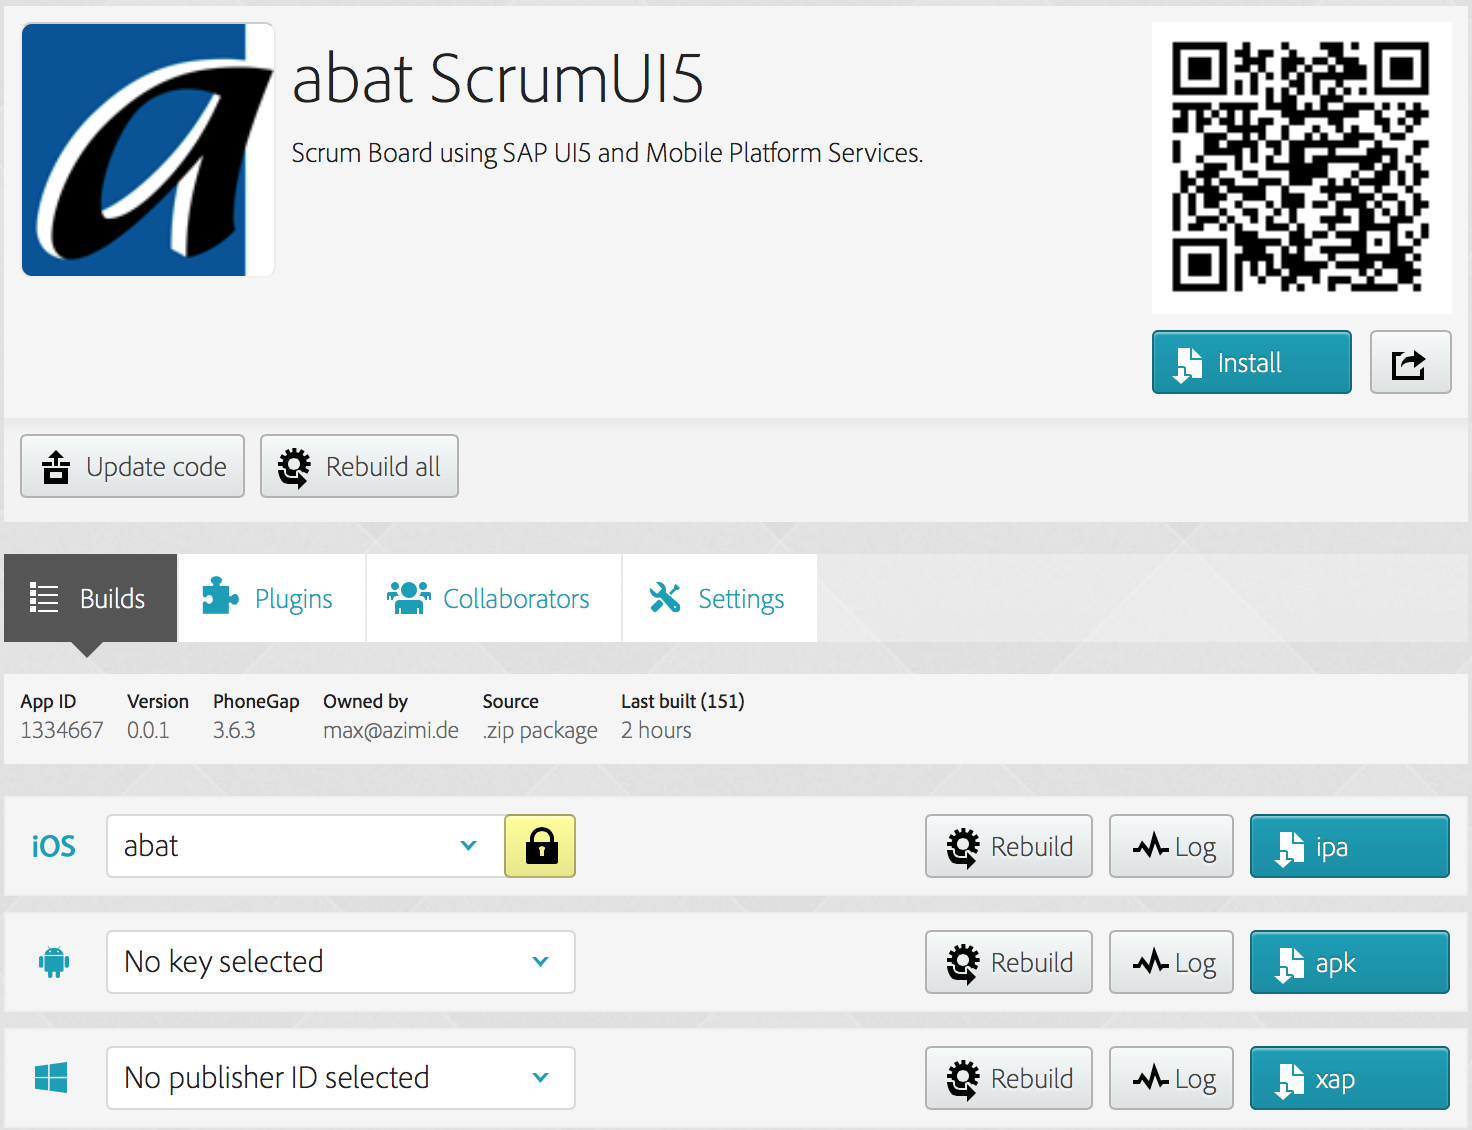
\includegraphics[width=.95\textwidth]{PhoneGapBuild}
\caption[PhoneGap-Build-Webinterface]{PhoneGap-Build-Webinterface.}
\label{fig:Phonegap}
\end{figure}

Die Konfiguration des PhoneGap Builds läuft über die Weboberfläche, die auf \autoref{fig:Phonegap} zu sehen ist. Der Quellcode der Web-Applikation kann als ZIP-Archiv gepackt und hochgeladen oder automatisch aus einem Git-Repository geladen werden. Anschließend wird die Anwendung für verschiedene Betriebssysteme direkt kompiliert und signiert. Für die Signierung der iOS-App müssen die  entsprechenden Entwicklerzertifikate hinterlegt werden.

Nach erfolgreichem Build der Anwendung können die Installationsdateien für die verschiedenen Plattformen heruntergeladen und für die weitere Verteilung genutzt werden. Zudem ist es möglich, die Anwendung über einen Link zu verteilen. Dieser installiert auf mobilen Geräten automatisch die App. 

Auf native Gerätefunktionen wird durch verschiedene Plugins zugegriffen, sodass Kamera oder GPS-Koordinaten auch für Web-Apps zugänglich sind. Durch das Kompilieren in der Cloud wird kein spezielles \ac{SDK} für die verschiedenen Plattformen wie iOS und Android benötigt. Es reicht eine Entwicklungsumgebung für Webanwendungen.

\autsubsection{JS Task Runner Grunt}{Azimi}
Um die Vielzahl an Werkzeugen für unseren automatischen Build aufzurufen, kommt der sogenannte JavaScript Task Runner Grunt\footnote{\url{http://gruntjs.com/}} zum Einsatz. Einzige Aufgabe ist die Abarbeitung der einzelnen Tasks, die in der Grunt-Konfiguration (siehe Listing \ref{lst:gruntfile}) definiert werden \cite[S.\ 59-61]{Wrobel2015}. Die eigentlichen Funktionalitäten sind in diverse Grunt-Plugins ausgelagert, die wir im Folgenden erläutern.

\begin{listing}
	\inputminted{javascript}{src/gruntfile-short.js}
	\caption{Auszug Gruntfile.js}
	\label{lst:gruntfile}
\end{listing}

\subsubsection{grunt-contrib-uglify}
Dies ist ein Grunt-Plugin zum Ausführen des UglifyJS-Toolkits. Hiermit wird der JavaScript-Code komprimiert, Variablennamen werden, wenn möglich, verkürzt und vorhandene Kommentare gelöscht. Die minified-JavaScript-Files besitzen typischerweise nur noch 30--40\,\% der Ursprungsgröße.
%  \cite{Uglify2015}

\subsubsection{grunt-eslint}
Überprüft den JavaScript-Code auf Einhaltung der vereinbarten Regeln zur statischen Code-Analyse per ESLint, einer Weiterentwicklung von JSHint. Hierfür stellt SAP im OpenUI5-Repository eine ESLint-Konfigurationsdatei zur Verfügung, die in eigenen Projekten verwendet werden kann \cite{SAP2015_2}.

\subsubsection{grunt-karma}
Dieses Plugin ermöglicht es, Karma während des Build-Prozesses aufzurufen. Über separate Karma-Tasks werden die Unit- und Akzeptanztests ausgeführt. \cite[S.\ 129-130]{Wrobel2015}.

\subsubsection{grunt-contrib-copy}
Verschiebt Dateien, \zB vom Source- in den Destination-Ordner.

\subsubsection{grunt-contrib-compress}
Komprimiert den Target-Ordner in einer ZIP-Datei, damit diese anschließend vom PhoneGap-Build-Plugin weiterverarbeitet wird.

\subsubsection{grunt-phonegap-build}
Lädt das in einer ZIP-Datei archivierte Projekt über ein \ac{API} zu PhoneGap Build. Anschließend löst es einen neuen Build aus und signiert die Installationsdateien.

\subsubsection{grunt-plato}
Neben der statischen Code-Analyse durch ESLint gibt es weitere Analysen des Quelltextes durch das plato-Plugin. Es stellt verschiedene Metriken zur Komplexität und Wartungsfreundlichkeit des Codes bereit.
%https://github.com/jsoverson/grunt-plato
%http://de.slideshare.net/JarrodOverson/complexity-28214103
%HIER MEHR SCHREIBEN!
\SuperPar
\SuperPar
\autsubsection{Jenkins}{Azimi}
Als Continuous-Integration-Server wird Jenkins\footnote{\url{https://jenkins-ci.org/}} eingesetzt. Für die Implementierung verschiedener Werkzeuge im Continuous-Integration-Prozess werden zusätzliche Plugins wie folgt verwendet:

\begin{figure}[h]
\centering
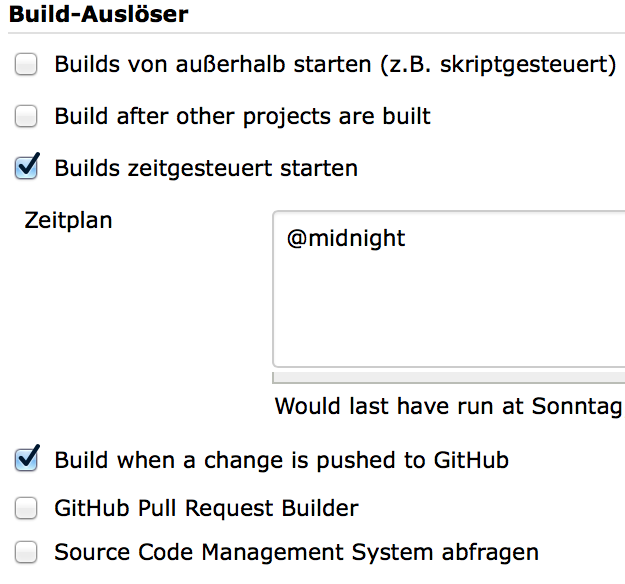
\includegraphics[width=.50\textwidth]{Github2-JenkinsConfig}
\caption[Build-Auslöser]{Build-Auslöser.}
\label{fig:Github2}
\end{figure}

\subsubsection{GitHub-Plugin}Zur Versionsverwaltung der Projektdaten wird GitHub verwendet. Das Plugin stößt den Build-Prozess bei Code-Änderungen im Repository automatisch an. Ebenfalls möglich ist eine zeitgesteuerte Ausführung oder ein manueller Start wie in \autoref{fig:Github2}. So ist gewährleistet, dass der Build inkl. Tests mit der aktuellen Version des Codes durchgeführt wird.

\subsubsection{Einbindung Paketmanager und Grunt}
Die Einbindung von Node.js, Bower und Grunt in den Continious-Integration-Prozess funktioniert durch Kommandozeilenbefehle, siehe \autoref{fig:Kommandozeile}, welche von Jenkins ausgeführt werden.

\begin{figure}[h]
\centering
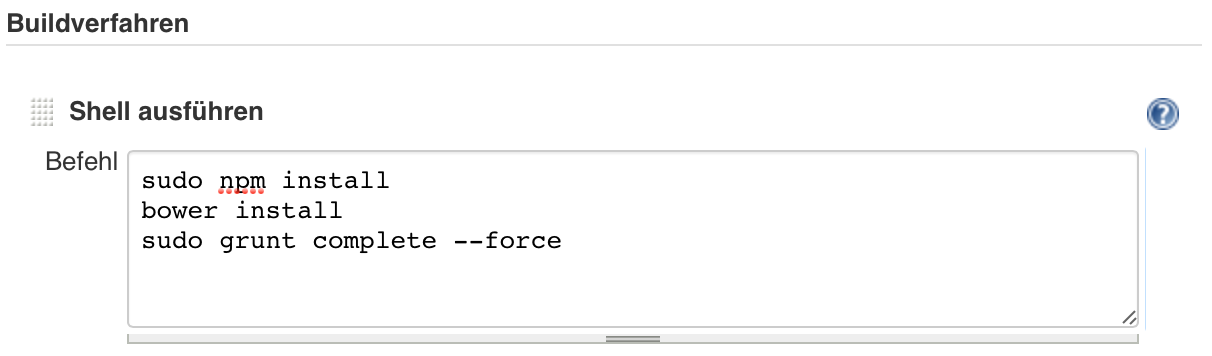
\includegraphics[width=.95\textwidth]{Kommandozeile}
\caption[Integration von Paketmanagern und Grunt]{Integration von Paketmanagern und Grunt.}
\label{fig:Kommandozeile}
\end{figure}


\subsubsection{Checkstyle}
Um die Ergebnisse des ESLint-Checks in Jenkins anzeigen zu können, wird das Jenkins-Checkstyle-Plugin genutzt. Dazu muss in der Jenkins-Projekt-Konfiguration der Pfad zu den Ergebnissen angegeben werden. Anschließend wird in der Projektübersicht ein Trend-Graph, wie in \autoref{fig:Checkstyle-Trendgraph} zu sehen ist, mit der Anzahl an Checkstyle-Warnungen erstellt. Zusätzlich lassen sich diese Warnungen je nach Verzeichnis, Datei oder Warnungs-Typ aufschlüsseln, vergleiche \autoref{fig:Checkstyle-Warnungen}.

\begin{figure}[h]
\centering
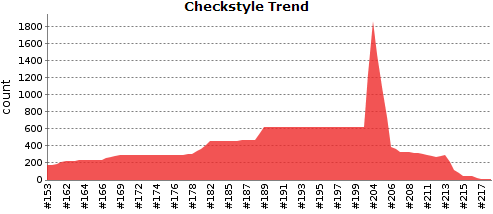
\includegraphics[width=.95\textwidth]{Checkstyle-Trendgraph} 
\caption[Checkstyle-Warnungen -- Trend-Graph]{Trend-Graph der Checkstyle-Warnungen.}
\label{fig:Checkstyle-Trendgraph}
\end{figure}

\begin{figure}[h]
\centering
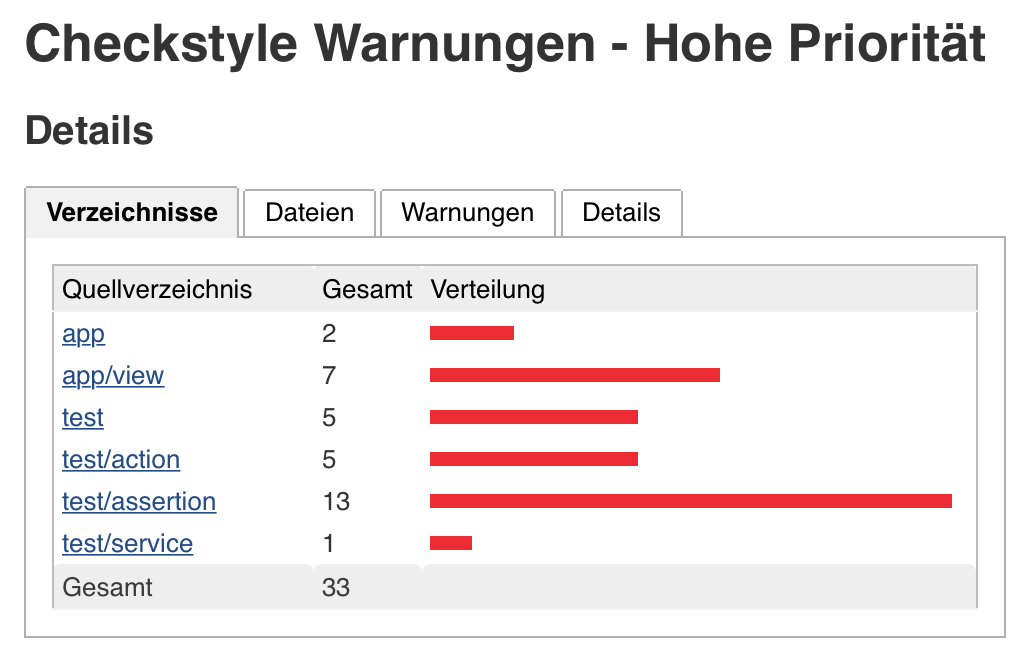
\includegraphics[width=.95\textwidth]{Checkstyle-Warnungen-high}
\caption[Checkstyle-Warnungen -- Hohe Priorität]{Checkstyle-Warnungen -- Hohe Priorität.}
\label{fig:Checkstyle-Warnungen}
\end{figure}

\subsubsection{Cobertura}
Zur Anzeige der Zeilenabdeckung aus den Akzeptanztests wird das Cobertura Plugin gebraucht. Das Plugin erzeugt einen Trend-Graphen, in dem die Zeilenabdeckung des Codes untergliedert in Pakete, Dateien, Klassen, Methoden, Zeilen und Verzweigung dargestellt wird, siehe \autoref{fig:CodeCoverage-Package}. Über den Graphen kann bis in die einzelnen Dateien und den dazugehörigen Quellcode navigiert werden. Welche Teile des Codes durch die ausgeführten Tests bisher abgedeckt bzw. eben nicht abgedeckt sind, wird hier nachvollziehbar, wie in \autoref{fig:CodeCoverage-Code} zu sehen ist.

\begin{figure}[h]
\centering
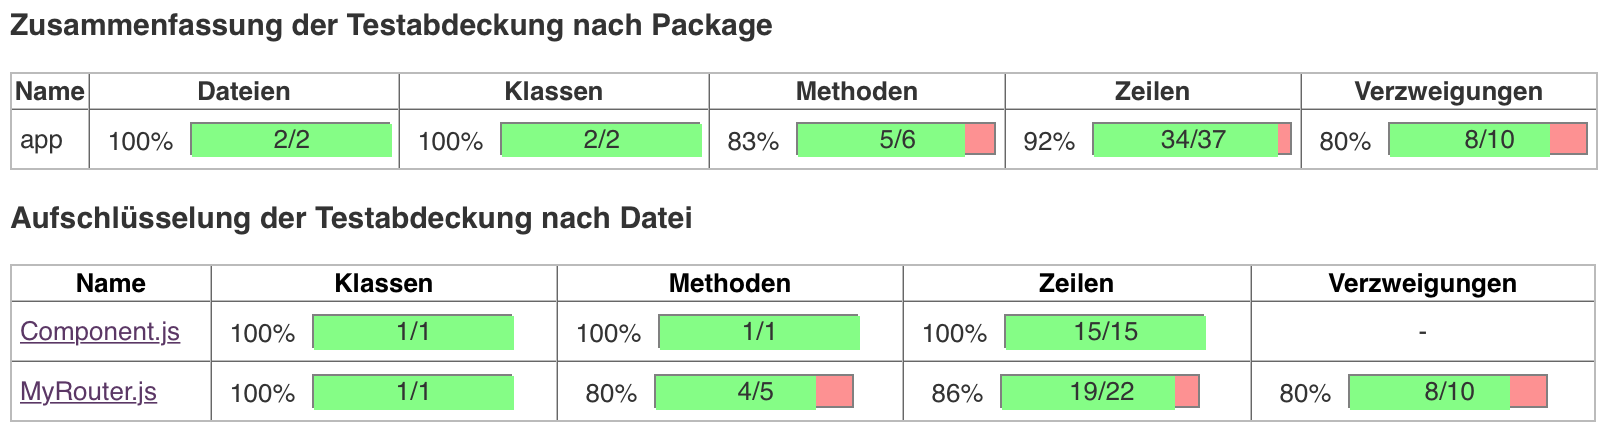
\includegraphics[width=1.25\textwidth]{CodeCoverage-Package}
\caption[Zeilenabdeckung im Paket \emph{app}]{Zeilenabdeckung im Paket \emph{app}.}
\label{fig:CodeCoverage-Package}
\end{figure}

\begin{figure}[h]
\centering
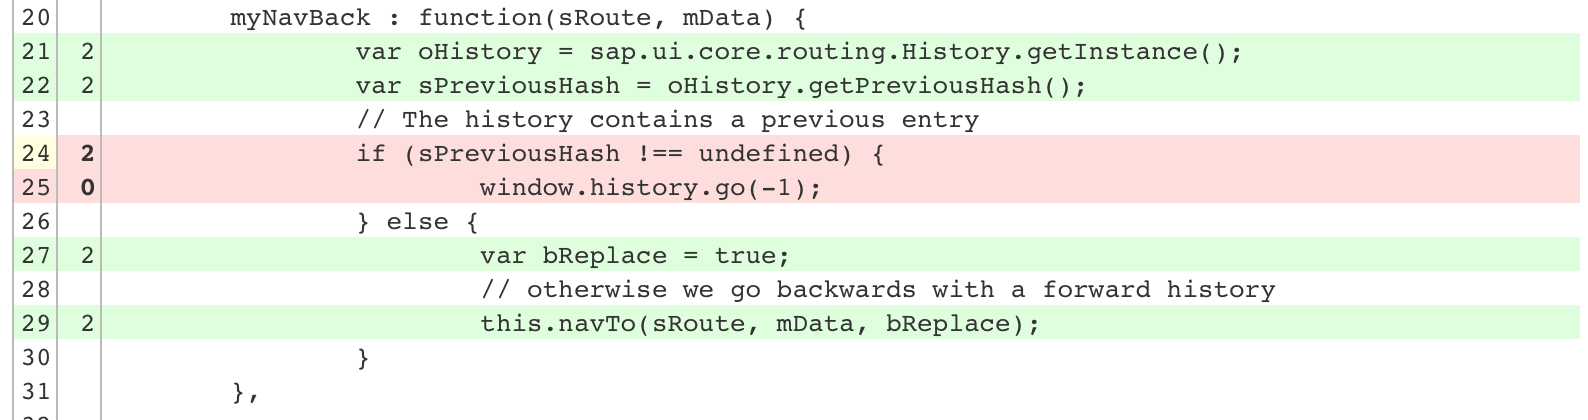
\includegraphics[width=1.25\textwidth]{CodeCoverage-Quellcode}
\caption[Zeilenabdeckung im Quellcode]{Zeilenabdeckung im Quellcode.}
\label{fig:CodeCoverage-Code}
\end{figure}

\subsubsection{HTML Publisher}
grunt-plato stellt die Ergebnisse der statischen Code-Analyse als HTML-Bericht zur Verfügung. Durch das Plugin wird in der Jenkins-Projektübersicht auf diesen Plato-Bericht verlinkt. Der Bericht zeigt Ergebnisse für das komplette Projekt oder auch für einzelne Dateien. In \autoref{fig:Platoresult} sieht man einen Report für die Datei Master3.controller.js.

\begin{figure}[h]
\centering
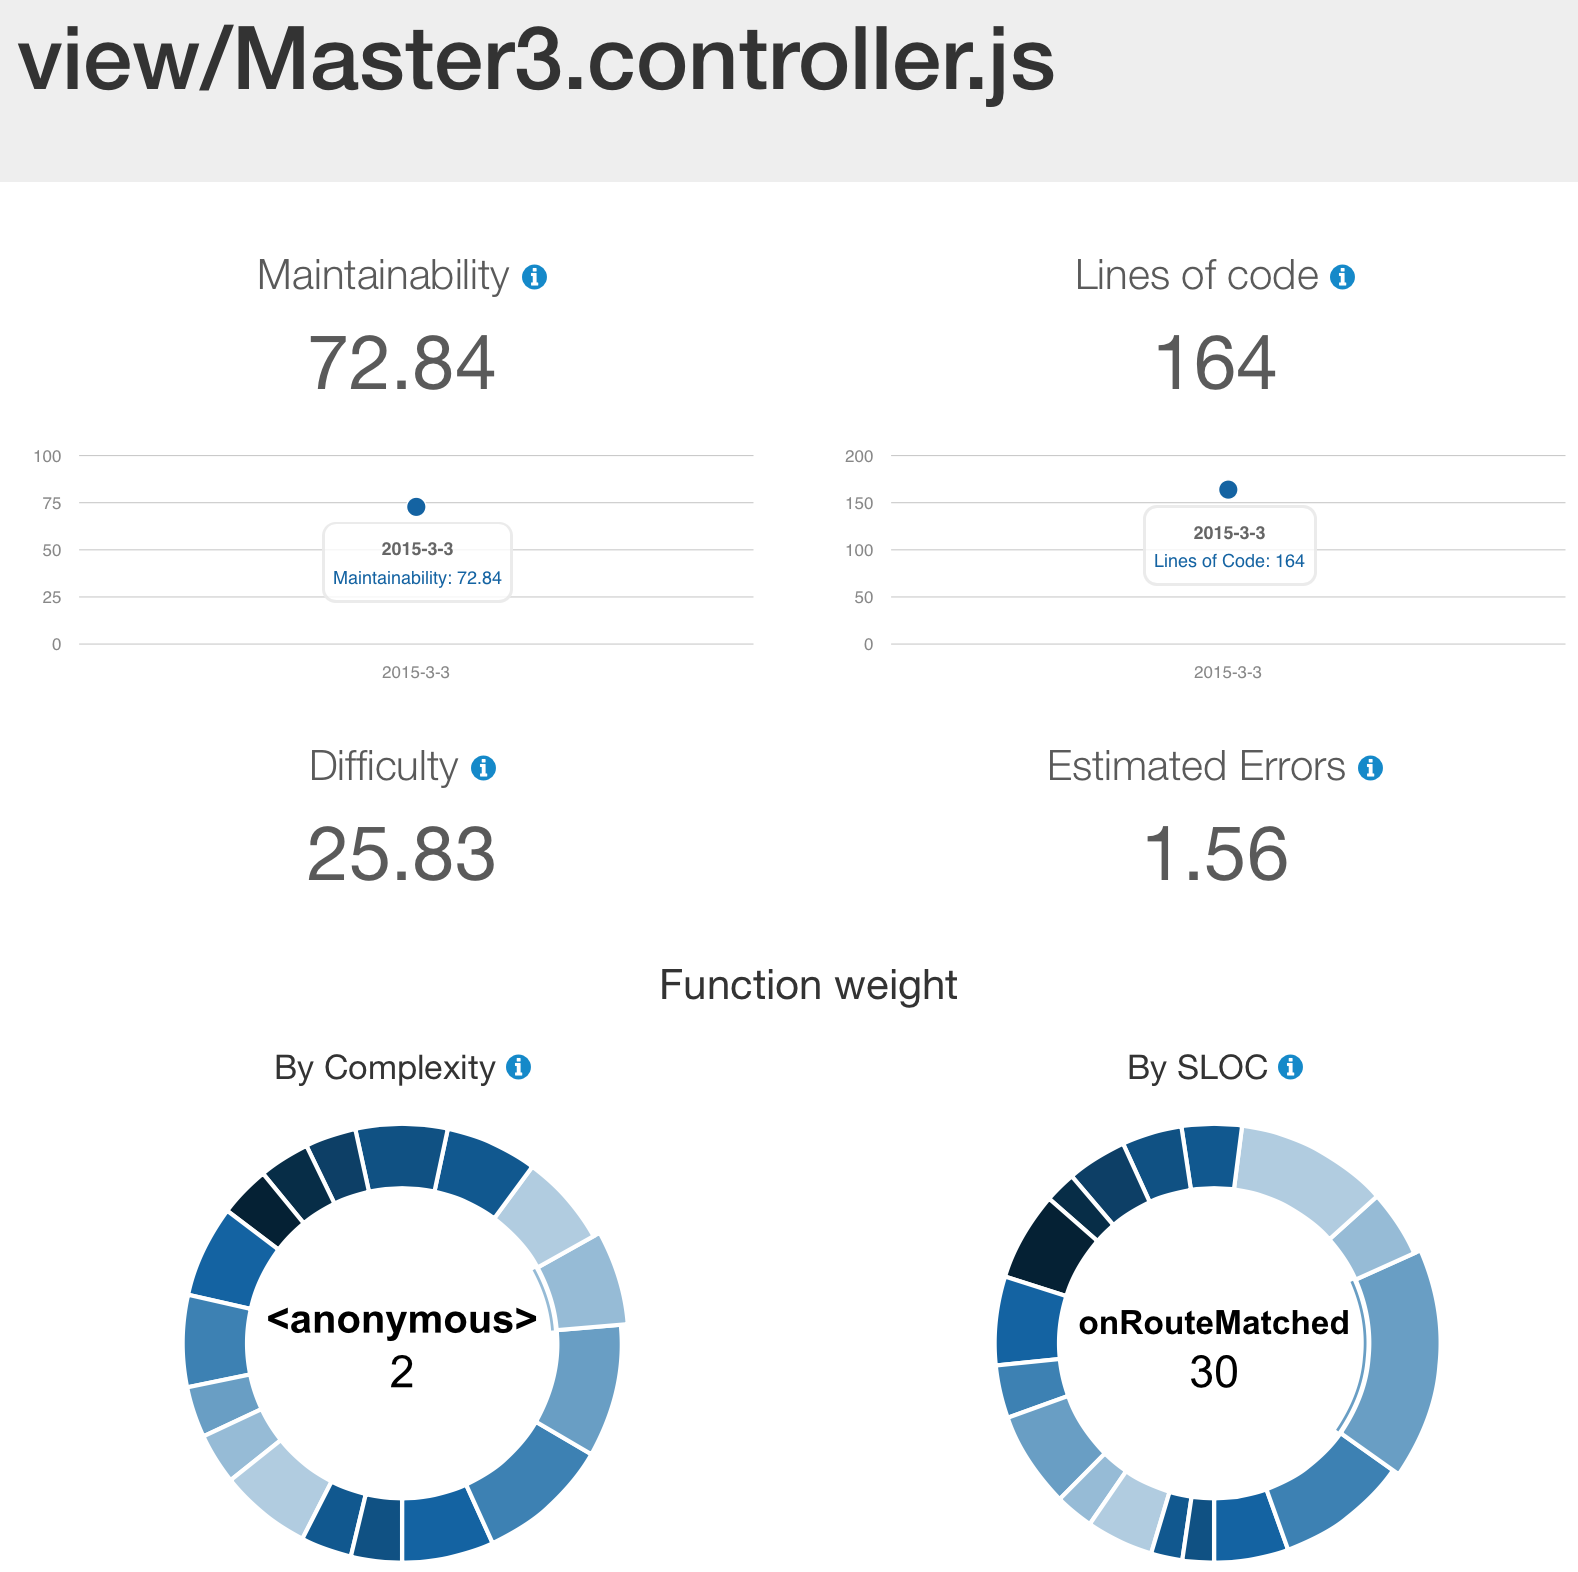
\includegraphics[width=.95\textwidth]{Plato2-JenkinsReport}
\caption[Plato-Bericht zu \emph{Master3.controller.js}]{Plato-Bericht zu \emph{Master3.controller.js}.}
\label{fig:Platoresult}
\end{figure}

\subsubsection{Timestamper}
Fügt der Konsolenausgabe von Jenkins einen Zeitstempel hinzu.

\subsubsection{Workspace Cleanup}
Ermöglicht das automatische Löschen des Arbeitsbereiches vor Ausführung des Builds. Da der komplette Prozess als Code abgebildet ist, wird permanent eine neue Build-Umgebung geschaffen.

% \begin{wrapfigure}[lines]{position}{breite}
\begin{wrapfigure}[4]{R}{2.5cm}
	\centering
	
\includegraphics{build_passing} 
	\caption[Build-Status]{Build-Status.}
	\label{fig:BuildStatus}
\end{wrapfigure}

\subsubsection{embeddable-build-status}
Erstellt ein Icon wie in \autoref{fig:BuildStatus} mit dem aktuellen Status des Builds zur Einbindung in Webseiten -- In unserem Fall in die GitHub Readme.

% Bugfix, Zeilennummern der Code-Listings sonst verschoben!
\begin{wrapfigure}[0]{l}{0cm}
\end{wrapfigure}

\newpage
\autsubsection{Zusammenfassung}{Azimi}
Die Testumgebung setzt sich aus drei großen Teilschritten zusammen. Diese sind die Build-Auslöser, der eigentliche Build-Prozess sowie die Post-Build-Operationen.

Build-Auslöser sind Ereignisse, die Jenkins dazu veranlassen einen neuen Build zu erstellen und alle Tests durchzuführen, die für dieses Projekt definiert wurden.
Dabei unterscheiden wir unter folgenden Build-Auslösern:
\begin{enumerate}
\item Der regelmäßige Build - jeden Tag um Mitternacht
\item Der Build bei Änderungen im GitHub - bei jedem Push
\item Der manuelle Start eines Buildvorganges
\end{enumerate}

Nach dem gemeldeten Ereignis durch den Auslöser startet Jenkins den Build. Zu Beginn jedes Builds wird der Arbeitsbereich gelöscht, um eine neue Build-Umgebung zu schaffen und die aktuelle Version des Quellcodes aus dem GitHub Repository herunterzuladen. Anschließend werden die benötigten Werkzeuge und Bibliotheken heruntergeladen und Grunt gestartet.

\SuperPar Im Build-Prozess werden schrittweise folgende Schritte ausgeführt:

\begin{enumerate}
\item Löschen des Arbeitsbereiches für einen sauberen Build
\item Code-Analyse durch ESLint und Plato
\item QUnit-Testausführung mit Karma inklusive Überprüfung der Zeilenabdeckung durch die QUnit bzw. OPA5-Tests
\item Kopieren der, für die App, notwendigen Dateien und Programmbibliotheken in den Target-Ordner
\item Komprimierung des JavaScript-Codes durch Uglify
\item Archivierung des Target-Ordners in eine ZIP-Datei
\item Hochladen der ZIP-Datei zu PhoneGap Build zum Kompilieren der Anwendung
\end{enumerate}

Zum Abschluss werden aus den Ergebnissen der verschiedenen Tests Berichte erzeugt und über die Jenkins-Oberfläche bereitgestellt. Die fertig kompilierte Anwendung lässt sich nun über PhoneGap Build auf den Geräten installieren. Die Dateistruktur des Projektes sieht nun so aus:

\begin{itemize}
	\item app/
	\item bower\_components/
	\item node\_modules/
	\item target/	
	\item test/
	\item test-reports/
	\item .eslintrc
	\item .gitignore
	\item bower.json
	\item config.xml
	\item Gruntfile.js
	\item karma.conf.js	
	\item package.json
\end{itemize}
\autsection{UI5-App}{Mattfeld}
\subsection{Auswahl der Entwicklungsumgebung}
\label{sec:auswahl_ide}

\subsubsection{Das bietet SAP}
Die von der SAP vorgeschlagene Universal-Entwicklungsumgebung ist Eclipse. Sie gehört \textit{noch} zur Firmenstrategie und wird mit einigen Plugins\footnote{\url{https://tools.hana.ondemand.com/}} einsatzbereit für die Entwicklung im SAP-Umfeld gemacht. Sie unterstützt unter anderem 
\begin{itemize}
	\item ABAP Development Tools for SAP NetWeaver
	\item SAP HANA Cloud Platform Tools
	\item Gateway (SAP Mobile Platform Tools)
	\item UI Development Toolkit for HTML5
\end{itemize}
Über die Transaktion \textit{/UI5/UI5\_REPOSITORY\_LOAD} werden UI5-Apps als \ac{BSP} auf einem SAP Web Application Server bereitgestellt. Das ist die Standard-Methode für Fiori-Apps. Die Transaktion ist remotefähig und wird per HTTP-Aufruf in eine CI-Toolchain eingebunden. Die gleiche Deploymentfunktion in Eclipse stellt der ABAP Repository Team Provider bereit.

Nicht zwingend notwendig, aber nützlich für die Backend-Entwicklung, ist der grafische OData Modeler aus den SAP Mobile Platform Tools, siehe \autoref{sec:OData-Modeler}. Er erleichtert Kommunikation und Abstimmung zwischen den Entwicklern. Die generierten Metadaten können sowohl im Gateway, als auch in SAPUI5 genutzt werden, ohne dass der eigentliche Service schon implementiert sein muss.

Das UI Development Toolkit for HTML5 enthält für die Frontend-Entwicklung:
\begin{itemize}
	\item App-Templates
	\item Test-Webserver
	\item Code-Vervollständigung
	\item XML-Syntaxprüfung
\end{itemize}
Ein schneller Einstieg in die UI5-Entwicklung ist mit diesen Tools möglich, sie sind jedoch keine Alleinstellungsmerkmale für Eclipse mit Plugin als \ac{IDE}. Sie sind auch in anderen Umgebungen verfügbar. Vielmehr sind die Templates für größere Projekte oder Nutzung als Fiori App durch fehlende Modularisierung sogar ungeeignet.

Noch schneller gelingt der Start mit der neuen SAP Web IDE\footnote{\url{http://scn.sap.com/docs/DOC-55465}}. Die Umgebung basiert auf Eclipse Orion und ist nach dem Login direkt startbereit. Dort sind modulare Templates für Fiori- und Hybrid-Apps verfügbar, die den aktuellen Best Practices folgen. Zu den weiteren Funktionen zählen:
\begin{itemize}
	\item Grafischer Layout-Editor 
	\item Live-Vorschau
	\item Code-Vervollständigung
	\item HANA Cloud Platform und ABAP-Repositories
	\item Mock-Daten-Support
\end{itemize}
Die ersten Erfahrungen mit der Web IDE sind vielversprechend: Die Anwendung reagiert schnell und implementiert außerdem anpassbare Code-Checks per ESLint und git-Support. Die Entwicklung schreitet schnell voran und soll auf lange Sicht Eclipse als UI5-IDE ablösen. 

Der Aufwand zur Entwicklung von Hybrid-Apps ist nicht verringert worden. Alle bekannten Build-Tools wie das Android SDK, Cordova, das Kapsel SDK u.\,a. müssen wie bisher lokal installiert und konfiguriert werden. Die Integration der Web IDE in externe Test- oder CI-Toolchains ist nicht möglich.

\subsubsection{Was benötigen wir?}
Wichtig sind möglichst wenig Kontextwechsel während der Entwicklung und damit eine hochintegrierte Entwicklungsumgebung. Das Werkzeug soll in den Hintergrund rücken und \ac{TDD} aktiv unterstützen. Wir wollen die gleiche Toolchain wie auf dem Integrationsserver nutzen.
Konkret benötigen wir:
\begin{itemize}
	\item Syntax-Hervorhebung der genutzten Sprache (JavaScript)
	\item Code-Vervollständigung der Frameworks (UI5)
	\item Integration von statischen Code-Analysen per ESlint
	\item QUnit-Testausführung per Karma
	\item Visualisierung der Code-Coverage
	\item Paketverwaltung per npm und Bower
	\item Grunt-Taskverwaltung
\end{itemize}
Eclipse beinhaltet im Auslieferungszustand nur wenig davon und die vorhandenen Funktionen wie Code-Vervollständigung in JavaScript-Projekten funktionieren nur selten. Manche der TDD-Funktionen ließen sich theoretisch per Plugin nachrüsten. Grunt als zentraler Task Runner aber \zB nicht. Da die vorhandene SAP-Integration allein Eclipse als IDE nicht rechtfertigt, wählen wir eine alternative IDE mit JavaScript- und TDD-Fokus.

\subsubsection{Lösung: WebStorm}
Gerade unter Web-Entwicklern genießt JetBrains WebStorm\footnote{\url{https://www.jetbrains.com/webstorm/}} einen hervorragenden Ruf: Die IDE ist speziell auf JavaScript-Projekte angepasst und bringt, neben zahlreichen Plugins, eine sinnvolle Vorkonfiguration mit. Schon aus früheren Projekten ist uns auch die Reaktionsfreude der zugrunde liegenden IntelliJ-Plattform bekannt. Wie können die bisher Eclipse-exklusiven Funktionen genutzt werden?

Die Syntax-Püfung von XML-Views ist über die entsprechenden XML-Definitionen (*.xsd) verfügbar. Diese sind Bestandteil des UI5 Development Toolkits for Eclipse, aber auch separat auf GitHub erhältlich\footnote{\url{https://github.com/jbmurray/UI5-WebStorm-Files}}. Das gleiche Repository enthält Bibliotheken, die sich für die UI5-Code-Vervollständigung in WebStorm nutzen lassen.
%\footnote{\url{http://scn.sap.com/community/developer-center/front-end/blog/2014/09/22/configuring-jetbrains-webstorm-for-ui5-development}}

Das ABAP Team Repository kann nicht integriert werden. Einchecken als \ac{BSP} aus WebStorm ist nur über den externen Aufruf einer Transaktion möglich. Für Fiori-Apps ist das verschmerzbar, da der CI-Server das finale Deployment übernimmt. Für hybride Apps spielt es ohnehin keine Rolle -- Installationspakete werden auf anderen Wegen verteilt, \zB über die App Stores oder eine \ac{MDM}-Lösung wie SAP Afaria.

\begin{figure}[h]
	\centering
	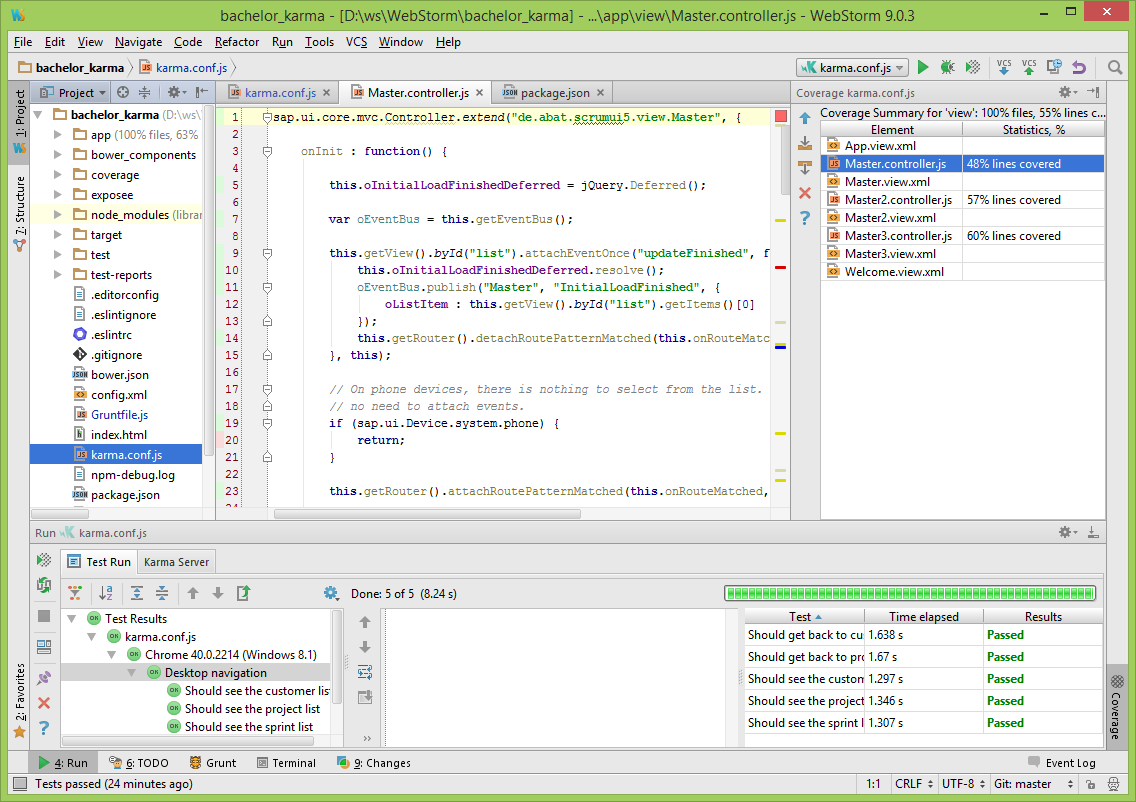
\includegraphics[width=1.25\textwidth]{WebStorm} 
	\caption[WebStorm mit TDD-Integration]{WebStorm mit TDD-Integration.}
	\label{fig:WebStorm}
\end{figure}

Webstorm integriert alle geforderten \ac{TDD}-Funktionen. \autoref{fig:WebStorm} zeigt die Ausführung von Karma-Tests in der \ac{IDE}. Test-Status und Code-Abdeckung werden direkt im Quellcode visualisiert. Grün markierte Zeilen wurden getestet, rote nicht. Um die testgetriebene Entwicklung in einer neuen WebStorm-Installation fortzusetzen sind folgende Schritte nötig:
\begin{enumerate}
	\item Klonen des Projekt-Repositories
	\item Installieren der Entwicklungs-Abhängigkeiten per \emph{npm install}
	\item Installieren der Frontend-Abhängigkeiten per \emph{bower install}
\end{enumerate}
Die Test-Konfiguration muss nicht angepasst werden -- WebStorm nutzt die, bereits als Code vorliegende, CI-Toolchain mit ihren Grunt-Tasks automatisch. Die Toolchain wird nicht nur abgespielt, sondern kann auch mit IDE-Unterstützung bearbeitet werden. WebStorm hat eigene Paketverwaltungen für Node.js und Bower, die sich entsprechend nutzen lassen.

Auch viele der weiteren Konfigurationsdateien werden automatisch erkannt. Die statische Code-Analyse erfolgt parallel mithilfe der eigenen ESLint-Regeln. Automatische Code-Formatierung orientiert sich an der IDE-übergreifenden \emph{.editorconfig}. Selbst die \emph{.gitignore}-Konfiguration findet bei der Nachverfolgung lokaler Änderungen Verwendung.

Insgesamt wird die Entwicklung durch WebStorm aktiv unterstützt. Alles was automatisiert werden kann, wird es auch. Die Benutzererfahrung ist deutlich besser als unter Eclipse, wo vieles nur langsam oder gar nicht funktioniert. Gegenüber der SAP Web IDE ist die Integration und Weiterentwicklungsmöglichkeit der CI-Toolchain sehr gelungen.


\subsection{UI5-App}
Abbildung \ref{fig:app_main_screen} zeigt den Hauptbildschirm der entwickelten UI5-Scrum-App. Sie ist nach dem typischen Master-Detail-Konzept gestaltet: In der linken Master-View wird erst ein Kunde ausgewählt, dann ein Projekt und Sprint. Anschließend zeigt die große Detail-View rechts die entsprechenden Sprint-Daten. Die Ansicht ist responsive, wird bei kleineren Bildschirmen also automatisch angepasst.

\begin{figure}
	\centering
	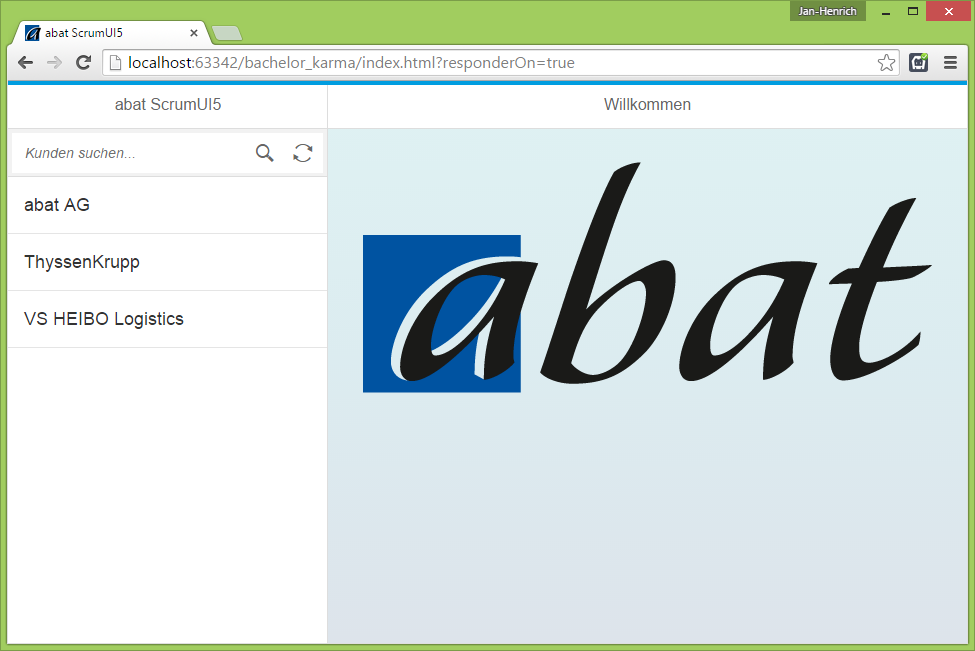
\includegraphics[width=0.95\textwidth]{app_main_screen} 
	\caption[UI5-App -- Hauptbildschirm]{UI5-App -- Hauptbildschirm mit Mock-Daten.}
	\label{fig:app_main_screen}
\end{figure}

Intern entspricht die App dem Model-View-Controller-Prinzip. Daraus ergibt sich folgende (gekürzte) Dateistruktur, die den aktuellen Best Practices entspricht:
\begin{itemize}
	\item app/
	\begin{itemize}
		\item i18n/
		\begin{itemize}
			\item messageBundle.properties
			\item messageBundle\_de\_DE.properties
		\end{itemize}		
%		\item img/
%		\begin{itemize}
%			\item background\_logo.png
%			\item favicon.ico
%		\end{itemize}
		\item view/
		\begin{itemize}
			\item Master.view.xml
			\item Master.controller.js
		\end{itemize}
		\item Component.js
		\item index.html
		\item MyRouter.js
	\end{itemize}
\end{itemize}

\subsubsection{Kapselung}
Als Startpunkt dient die \textit{index.html}, sie ermöglicht die Ausführung der App im Browser. Metatags geben dem Browser Hinweise zur korrekten Darstellung. Danach findet nur noch das Bootstrapping, also Laden, der UI5-Bibliotheken statt. Anschließend wird die App in einem Shell-Container gestartet.

Die eigentliche App ist unabhängig von einer HTML-Datei in der \textit{Component.js} definiert. Durch diese Kapselung ist die App portabel. Eine weitere Ausführungsumgebung ist \zB das Fiori Launchpad. In der Komponente sind allgemeine Informationen wie App-Name und Version gespeichert. Ebenso festgelegt ist die erste aufzurufende View.

\subsubsection{Routing}
Daneben enthält \textit{Component.js} die Routen-Konfiguration. Das Routing-Konzept ist Teil der Kapselung, da die Navigation innerhalb der App über einen eigenen Router (\textit{MyRouter.js}) stattfindet. In Ausführungsumgebungen mit mehreren UI5-Apps werden Konflikte vermieden.

Weiterer Vorteil: Über bestimmte URLs ist immer der gleiche App-Zustand erreichbar. Wie von anderen Webanwendungen gewohnt, kann über den Parameter \textit{/Kunden(Kunde='ABAT')/Projekte} immer die Projektübersicht des Kunden, in diesem Fall abat, aufgerufen werden. Die entsprechende Seite lässt sich bequem als Lesezeichen speichern.

\subsubsection{Internationalisierung}
Statische Texte sind in Resource Bundles wie \textit{messageBundle\_de.properties} definiert. Sie enthalten Schlüssel/Wert-Paare mit der entsprechenden Übersetzung in einer bestimmten Sprache und Landeskennung. Englische Standardtexte sind grundsätzlich in \textit{messageBundle.properties} gespeichert. 

In einer XML-View wird statischer Text wie \textit{i18n>masterTitle} automatisch mit dem Pendant aus dem i18n-Model ersetzt. Die aktuelle Sprache wird \zB aus dem Browser, dem Betriebssystem oder einem URL-Parameter bestimmt. UI5 sucht automatisch das passende Resource Bundle.

\subsubsection{OData}
Die Adresse des OData-Services ist ebenfalls in der \textit{Component.js} festgelegt. Während der Initialisierung werden die Metadaten geladen und als globales App-Model festgelegt. 
Anschließend werden die Elemente einer Liste \zB über \textit{items='{/Kunden}'} entsprechend der Einträge im Pfad des OData-Services angezeigt. 
Bei einem Klick auf den Kunden, wird dieser als aktueller \textit{BindingContext} gespeichert. Die Elemente der nachfolgenden Liste werden dann unter \textit{{gespeicherterKunde}/Projekte} gesucht. An dieser Stelle greifen UI5 und die Navigationseigenschaften des OData-Services ineinander.

\subsection{Akzeptanztests mit OPA5}
OPA5 basiert auf QUnit und ermöglicht Akzeptanztests für UI5-Apps. Es erleichtert die Test-Programmierung durch spezielle Selektoren für UI5-Controls und die Verwaltung von Asynchronität.

Analog zu den Testfall-Szenarien im \autoref{sec:tests} werden Tests per \textit{Given/When/Then} definiert. Die Formulierung aus den Testfällen lässt sich fast direkt in Code umsetzen, siehe Listing \ref{lst:opa5}. Voraussetzung hierfür ist die vorherige Definition zahlreicher eigener \textit{Actions} und \textit{Assertions}. 

Ein Beispiel ist die Assertion \textit{iShouldSeeTheCustomerList()}. Diese wird aus \textit{NavigationAssertions.js} nachgeladen und dem Framework über \textit{extendConfig()} bekannt gemacht. Innerhalb der nachgeladenen Datei ruft sie generellere Funktionen wie \textit{iClickOnAListItem(listName)} auf. Hierüber ist eine grundsätzliche Modularisierung der Tests möglich.

Nur für bestimmte Views nützliche Testfunktionen werden diesen über PageObjects zugeteilt und automatisch mitgeladen. Dies erleichtert die Strukturierung. Trotzdem wird das Testprojekt bei größerem Umfang schnell unübersichtlich. Die meisten Funktionen müssen selbst erstellt werden. Ein grafischer Editor, wie \zB Jubula ihn mitbringt, wäre von großem Vorteil.

Die OPA5-Tests können über eine HTML-Datei gestartet werden. Diese dient nur als Container, analog zum Start der normalen App-Komponente. Dort werden sie wie klassische QUnit-Tests in einem iFrame ausgeführt. In unserer Toolchain genügt eine JavaScript-Datei wie Listing \ref{lst:opa5}, die von Karma ausgeführt wird.

Die Implementierung des Mockservers ist bereits in \autoref{sec:karma} beschrieben. Er wird über den URL-Parameter \textit{?responderOn=true} aktiviert. Der Test läuft jetzt auch ohne Verbindung zum Backend.
%Die gekürzte Verzeichnisstruktur der Tests:
%\begin{itemize}
%	\item test/
%	 \begin{itemize}
%		\item actions/
%		\item arrangements/
%		\item assertions/
%		\item Navigations.js
%%		\item opaTests.qunit.html
%	\end{itemize}
%\end{itemize}

\begin{listing}[H]
	\inputminted[tabsize=2]{js}{src/opa5.js}
	\caption{OPA5-Test-Szenario 1}
	\label{lst:opa5}
\end{listing}

\chapter{Schlussfolgerungen}
\label{cha:Schlussfolgerungen}

\section{Lessons Learned}

\subsection{Architektur-Überlegungen}
Die Möglichkeiten eine UI5-App zu veröffentlichen und zu nutzen sind vielfältig. Da die geschaffene Infrastruktur meist längerfristig genutzt wird, sollte sie nicht nur zur konkreten App, sondern zur gesamten Firmenstrategie passen. Besonders interessant sind folgende Aspekte:

\begin{enumerate}
	\item Sind weitere UI5-Apps geplant?
	\item Werden Fiori-Apps genutzt?
	\item Existiert bereits eine MDM-Strategie?
	\item Verteilung und Update der Apps
	\item Aus welchem Netz erfolgen Zugriffe?
	\item Welche Authentifizierungsserver werden genutzt?
	\item Ist ein Offline-Zugriff nötig?
	\item Sind native Gerätefunktionen gefordert?
	\item Sollen eigene Plugins genutzt werden?
	\item Umfang des Brandings/CI
	\item Art und Standort der Backend-Systeme
	\item Ist Cloud-Infrastruktur gewünscht?
\end{enumerate}	
Diesen Stichpunkten folgend, können die passende Architektur und zugehörige Produkte ausgewählt werden. Zusätzlich ergeben sich Art und Umfang der Teststrategie und besonders der Testwerkzeuge.

\subsection{OData-Service generieren oder selbst implementieren?}
Bei geeigneten Schnittstellen ist die Generierung von OData-Services tatsächlich sehr gut geeignet, um schnell erste Ergebnisse zu liefern. So entsteht in kürzester Zeit ein funktionsfähiger Service mit grundlegenden Funktionen. Für die Erweiterung und Optimierung von generierten Services ist dennoch ABAP-Programmierung nötig. 

Ohne bereits vorhandene Schnittstellen oder bei komplexen Services empfiehlt es sich, direkt zur Selbstimplementierung des Services zu greifen, auch wenn der Initialaufwand etwas höher ist. 

Die Entwicklung für das SAP-Backend lief, dank umfassender Dokumentation, gut. Der Aufwand steigt erheblich, sobald von Standard-Funktionen abgewichen wird und Customizing notwendig wird. \ZB das Filtern von Substrings bei Nichtbeachtung der Groß- und Kleinschreibung kann nicht über die bereitgestellten Standard-Methoden zum Auslesen von übergebenen OData-Parametern genutzt werden. 

Insgesamt verschiebt sich der Aufwand hin zur Backendprogrammierung. Jede dort implementierte Funktion vereinfacht die Entwicklung der UI5-App. Ein gutes Beispiel sind die Navigationseigenschaften des OData-Modells. Sind sie korrekt implementiert, genügt im Frontend die korrekte Verlinkung, weitere Logik muss nicht implementiert werden.


\subsection{Wo ist die aktivste UI5-Community?}
Mit der Veröffentlichung des UI5-Codes auf GitHub verschieben sich auch die Anlaufstellen für Fehlermeldungen und Hilfestellungen. Während der Kontakt zu den Framework-Entwicklern vor OpenUI5 kaum möglich war, können Fehlermeldungen oder Hinweise nun direkt über das GitHub Issue Management eingestellt werden. Zum Beispiel im Fall des fehlerhaften \textit{karma-openui5} Plugins hat sich so ein interessanter Dialog ergeben. Der veröffentlichte Code gewährt außerdem Einblicke in zukünftige Best Practices in Form neuer Beispiel-Apps und den zugehörigen Testfällen.

Das SAP Community Network (SCN)\footnote{\url{http://scn.sap.com/community/developer-center/front-end}} ist weiterhin die wertvollste Ressource für Blogs und umfangreiche Tutorials. Auch komplexe Themen, wie das Kapsel SDK, werden mit Beispielen eingeführt und erleichtern den Entwicklungsstart ungemein. Daneben könnte StackOverflow als renomiertes Programmier-Forum nützlich werden. Die Zahl der Posts unter den Tags \textit{openui5} und \textit{sapui5}\footnote{\url{http://stackoverflow.com/questions/tagged/sapui5}} nimmt ständig zu.

\subsection{Infrastruktur als Code}
Das Prinzip \textit{Infrastructure as Code} ist nicht nur essenziell für die verteilte testgetriebene Entwicklung, es wird durch den hauptsächlichen Einsatz von JavaScript auch erheblich gefördert. Die gesamte Toolchain von Task Runner über Paketmanager und Testtreiber wird automatisiert aus den Konfigurationsdateien wiederhergestellt. 

Selbst beim erstmaligen Herunterladen aus der Versionskontrolle ist das Projekt in IDE oder CI-Server mit zwei Befehlen einsatzbereit.
Auf dem CI-Server machen wir uns diese Eigenschaft zunutze, indem das Projektverzeichnis vor jedem Build neu aufgebaut wird. Mögliche Nennwirkungen werden vermieden und die Lauffähigkeit der aktuell eingecheckten Infrastruktur ist sichergestellt.

\subsection{Alternative IDE prüfen}
Auch wenn SAP Eclipse als Standard-Entwicklungsumgebung für fast alle Produkte präsentiert -- Für eine UI5-Entwicklung auf JavaScript-Basis gibt es interessante Alternativen mit hervorragender Testintegration. 

Eclipse ist keine beliebte Webentwicklungsumgebung, laut SCN\footnote{\url{http://scn.sap.com/community/developer-center/front-end/blog/2014/09/22/configuring-jetbrains-webstorm-for-ui5-development}} auch nicht innerhalb der SAP. Hinzu kommt die neue SAP Web IDE als Konkurrenz und langfristige Ablösung einer lokalen Eclipse-Installation. Ihr erster Eindruck ist gut: Die Umgebung ist sofort einsatzbereit, reagiert schnell auf Eingaben, bringt aktuelle, Fiori-kompatible Templates mit und integriert statische Code-Analysen. Einzig die Entwicklung von hybriden Apps wurde nicht vereinfacht, die CI-Integration ist noch gar nicht möglich.

Je nach eigenen Vorlieben und Projektvorgaben kann WebStorm eine gute Alternative zu Eclipse und der Web IDE sein. Genauso wie Letztere ist WebStorm schnell einsatzbereit und arbeitet zügig. Zusätzlich können auch Unit- und Akzeptanztests ausgeführt und Ergebnisse visualisiert werden. Paketmanager sind integriert und auf Wunsch läuft die gesamte CI-Toolchain lokal in der IDE. Gerade in Hinblick auf TDD ist die Benutzererfahrung mit WebStorm wesentlich besser.

\subsection{Testmethoden kombinieren}
TDD stellt sicher, dass der Code richtig geschrieben wurde, während BDD dafür sorgt, dass es auch der richtige Code ist.
Ergänzend haben sich explorative Tests als nützlich erwiesen. 

Diese sollten allerdings nicht nur spontan, sondern in Form bestimmter Szenarien oder Aufträge erfolgen. Ein Auftrag könnte lauten: \textit{Überprüfe die Navigation in der App}. Sollten hierbei neue Fehlerwirkungen auftreten, schreiben wir einen entsprechenden Testfall und korrigieren den Code erst danach. Durch automatische Regressionstests wird der Fehler zukünftig vermieden.

\subsection{Tests gezielt einsetzen -- Nicht doppelt testen}
Durch die Offenlegung des UI5-Quellcodes auf GitHub ist die testorientierte Entwicklung seitens SAP deutlich geworden. Das gesamte Framework ist durch zahlreiche Unit- und Akzeptanztests geprüft. Gleiches gilt für die zugrundeliegenden Basis-Frameworks wie jQuery und QUnit. 

Probehalber haben wir die UI5-Tests ausgeführt -- Der mehr als 15 Minuten dauernde Testlauf endete mit mehreren Fehlermeldungen und Warnungen. Was bedeutet das für unser Projekt?

\begin{enumerate}
	\item Auch UI5 ist natürlich nicht fehlerfrei.
	\item Keiner der fehlgeschlagenen Testfälle ist für uns relevant.
	\item Teilweise sind noch nicht implementierte Funktionen betroffen.
	\item Der gesamte Testlauf dauert sehr lange.
	\item Die Ergebnisanalyse ist extrem aufwändig.
\end{enumerate}
Wir konzentrieren uns daher auf Tests eigener Funktionen.

\subsection{Statische Analyse differenziert betrachten}
Die Bereitstellung offizieller UI5-ESLint-Regeln zur statischen Codeanalyse ist der richtige Schritt, um die Code-Qualität zu verbessern und den gleichen Code-Stil projektübergreifend durchzusetzen. 

Das aktuelle UI5-Framework genügt diesen selbst gesetzten Anforderungen jedoch nicht: Eine Überprüfung mit ESLint zeigt so viele Warnungen, dass mit einem kompletten Refactoring auf absehbare Zeit nicht zu rechnen ist. Daraus folgern wir für unsere Projekt:
\begin{enumerate}
	\item Die genutzten Frameworks von der statischen Analyse ausschließen.
	\item Für zukünftige Kompatibilität eigenen Code regelkonform gestalten.
\end{enumerate}
Bei der Übernahme einer bereits vorhandenen Codebasis ohne fest definierte Regeln kann kaum ein bestimmtes Regelset durchgesetzt werden. Die Änderungen sind oft viel zu umfangreich und kommen einer Neuprogrammierung nahe. Stattdessen empfiehlt sich die Suche nach einem Stil der möglichst genau dem des vorhandenen Codes entspricht und eine Anpassung ermöglicht.

Im Notfall ist die Gewichtung der Fehler per Regel herunterzusetzen oder bestimmte Optionen ganz zu deaktivieren. Neue Fehler gehen sonst im Protokoll unter. Eine statische Analyse die standardmäßig viele Warnungen ausgibt, stumpft ab und bringt keinen Mehrwert.

\subsection{Code Coverage ist nicht alles}
Die Code Coverage ist zwar leicht zu messen, aber keine geeignete Metrik um das erfolgreiche Testende festzustellen. Stattdessen liefert sie Hinweise auf ungenutzten Code, der durch ein Refactoring entfernt werden kann.

Für die Wartbarkeit haben sich die Plato-Metriken als interessant herausgestellt. Sie analysieren die Komplexität des Codes und decken Modularisierungspotential auf.

%\subsection{Tests modularisieren}
%OPA5-Templates anlegen und Tests modularisieren % Gleiche Standards wie Code
%Vergleich mit Jubula % TEstdaten, graifschie Modularisierung, Generalisierung, (Komplizierter mit OPA5, einzelne JS files, selber Überblick behalten dafür Interface schnelelr (texteditor)), 

\section{Ausblick}
Es bleibt ein breit gefächertes Integrationspotenzial. Während die Arbeit eine Einführung in TDD und CI mit UI5 darstellt, bleiben weitere Funktionen, App-Architekturen und Testwerkzeuge die, je nach Projektart und Größe, weiter untersucht werden sollten.

\subsection{\emph{Echte} Unit-Tests}
Wie bereits festgestellt, handelt es sich bei unserer beschriebenen Vorgehensweise aktuell nicht um klassisches \ac{TDD} mit Unit-Tests -- Vielmehr nutzen wir Akzeptanztest.

Dieses Vorgehen hat sich bei der kleinen Projektgröße und dem geringen Umfang der App bewährt. Sobald eigene Funktionen in der App implementiert werden, zum Beispiel Formatter, werden Unit-Tests benötigt.

Mit der aktuellen Architektur haben wir alle Grundlagen dafür gelegt. QUnit als Testframework ist bereits UI5-Bestandteil und wird von unserem Testtreiber unterstützt. Auch die übrige CI-Toolchain ist auf den Einsatz vorbereitet.
%
%\subsection{Weitere App-Architekturen}
%SAP-App-Architekturen testen, siehe Überblick. 

\subsection{Native Funktionen testen}
Zukünftige App-Versionen werden native Geräte-Funktionen nutzen. Auch diese müssen in die Teststrategie einbezogen und automatisch geprüft werden. Aktuell gibt es für einen Test ohne Mobilgeräte oder Emulatoren folgende Möglichkeiten:

\begin{itemize}
	\item Browser-Plugins\footnote{\url{https://github.com/pbernasconi/chrome-cordova}}
	\item Mock-Frameworks\footnote{\url{https://github.com/ecofic/ngCordovaMocks}}
	\item Cordova-Browser-Plattform\footnote{\url{https://github.com/apache/cordova-browser}}
\end{itemize}
Cordova-Browser-Plugins und -Mock-Frameworks arbeiten nach dem gleichen Schema: Sie bieten einen Mock der cordova.js-API an. Dieser wird entweder direkt in den Testressourcen eingebunden oder in eine laufende Browsersitzung injiziert. API-Aufrufe liefern vordefinierte Werte oder zeigen einen Dialog zur Eingabe der Testdaten.

Die vielversprechendste Möglichkeit ist die neue, offizielle Cordova-Platt\-form \textit{Browser}. Sie ist seit 2014 als Beta-Version verfügbar und ermöglicht einen problemlosen Betrieb von Hybrid-Apps in Desktop-Umgebungen. Das \textit{deviceready}-Event wird automatisch abgesetzt und Standard-APIs wie Kamera und GPS stehen zur Verfügung. Aktuell ist die Einrichtung allerdings noch aufwändig.

\subsection{Tiefere SMP-Integration}
Aktuell nutzen wir die SAP Mobile Platform in Form der HANA Cloud Platform mobile services: Sie stellt unseren OData-Service außerhalb des Intranets bereit. Zusammen mit den Cordova-Plugins des Kapsel-SDKs bietet es noch mehr Möglichkeiten\footnote{\url{http://scn.sap.com/docs/DOC-49592}}:

\begin{itemize}
	\item Single Sign-on
	\item OData-Offline-Funktionen
	\item Push-Nachrichten
	\item App-Updates
	\item Statistiken
\end{itemize}
Gerade Single-sign on ist für eine zukünftige Mobil-Strategie auf UI5-Basis Voraussetzung, um mehrere Apps komfortabel nutzbar zu machen. Statt des SAP-Kontos als Fiori-Standard, können über die Mobile Platform auch andere Authentifizierungsstrukturen eingebunden werden, zum Beispiel ein Active Directory.

Offline-Funktionen stellen für die App-Entwicklung eine große Herausforderung dar. Die Eigenimplementierung von Synchronisierungsfunktionen ist komplex und damit fehleranfällig. Hier unterstützt die Kombination aus SAP Mobile Platform und Kapsel-Plugin -- Sie erweitert auch vorhandene OData-Services und UI5-Apps unter iOS und Android um Offline-Funktionen. Gleiches gilt für Push-Nachrichten.

Automatische App-Updates können für bereits installierte Apps über die Mobile Platform veröffentlicht werden. Dies kann allerdings nur eine Ergänzung zu einem vorhandenen Mobile Device Management wie Afaria sein. Nur darüber gelingt die Erstverteilung.

\subsection{Fiori Deployment}
Durch die strikte Einhaltung der UI5-Best-Practices eignet sich die App auch zur Veröffentlichung über Fiori: Die Modularisierung ermöglicht einen Betrieb der App allein über das Laden der \textit{Component.js}. Ob dies über eine HTML-Datei oder im Fiori-Launchpad erfolgt, spielt keine Rolle. Ressourcen und Navigations-Routen der App sind gekapselt und garantieren einen konfliktfreien Betrieb als Fiori-App.

In diesem Zusammenhang muss die parallele Veröffentlichung über das Fiori-Launchpad als BSP weiter geprüft werden. Ein manueller Upload der App widerspricht dem CI-Gedanken. Der ABAP Team Provider (Eclipse) oder das Aufrufen der Transaktion \textit{/UI5/UI5\_REPOSITORY\_LOAD} scheiden als Werkzeuge aus. Da der Baustein remotefähig ist, könnte eine CI-Integration über einen RFC erfolgen.

\subsection{Continuous Delivery mit Afaria}
Entwicklungs- und Testprozess sind automatisiert, doch wie kommt die Anwendung danach auf die mobilen Geräte der Mitarbeiter?

SAP bietet mit Mobile Secure eine \ac{EMM}-Lösung in der Cloud. Diese stellt durch die Integration von SAP Afaria unter anderem \ac{MDM} zur Verwaltung von mobilen Geräten im Unternehmen bereit. Außerdem werden per \ac{MAM} Anwendungen im firmeninternen App Store über den \textit{SAP Mobile Place} veröffentlicht. 

Durch Schnittstellen lassen sich die Installationspakete der Apps direkt aus der CI-Toolchain im \textit{SAP Mobile Place} bereitstellen. Die Mitarbeiter oder auch Geschäftspartner können Anwendungen anschließend aus dem Anwendungskatalog auswählen und installieren. Auf Geräten, die durch das \ac{MDM} verwaltet werden, ist außerdem eine automatische Installation und Aktualisierung der Anwendungen möglich. Alternativ ist SAP Afaria auch als Stand-Alone-Lösung einsetzbar\footnote{\url{http://scn.sap.com/docs/DOC-62378}}. 

\subsection{eCATT-Integration}
Das Testen der Funktionsbausteine, sowie der OData-Services wurde in diesem Projekt aus Zeitgründen nicht automatisiert. Dies würde sich über das \ac{eCATT} realisieren lassen. 

Die Funktionen zum Testen von Funktionsbausteinen ist standardmäßig in \ac{eCATT} integriert. Automatisierte Tests von OData-Services benötigen zusätzlich die \textit{Gateway Test APIs}, welche im SCN veröffentlicht wurden\footnote{\url{http://scn.sap.com/community/gateway/blog/2013/11/27/ecatt-based-test-automation-for-odata-services-available}}.

\section{Bewertung und Herausforderungen}
Ziel der Arbeit war ein bereits vorhandenes ABAP-Altsystem mit einer neuen UI5-App benutzerfreundlicher zu gestalten. Wir haben dabei die neue SAP-Mobile-Strategie eingeschätzt und die entsprechenden Produkte kennengelernt. Seit der Sybase-Übernahme durch SAP wurde die ehemalige Sybase Unwired Platform zur SAP Mobile Platform weiterentwickelt -- Mittlerweile auch als Mietangebot in Form der Hana Cloud Platform mobile services. Überhaupt existiert nun ein großes Ökosystem zum Thema Mobile Devices das \zB um MDM-Lösungen erweitert wurde. In dieser Arbeit haben wir die gängigste Kombination aus universeller UI5-App und SAP Gateway umgesetzt.

Gegenüber älteren Frameworks wie jQuery Mobile ist UI5 ein vollwertiges, offenes Businessframework. Übliche Konzepte wie Routing, Internationalisierung und Modularisierung heben es auf eine Stufe mit großen Alternativen wie Sencha Ext JS. Die typische Schnelllebigkeit anderer JavaScript-Frameworks lässt sich auch hier beobachten: Die eigenen Codestyle-Vorgaben werden noch nicht eingehalten und sind eher Ziel, als aktueller Standard. Die interne App-Struktur hat mehrere grundlegende Änderungen durchlaufen, die Best Practices werden das nächste Mal mit dem kommenden Release 1.28 umfassend geändert.

Das Konzept des SAP Gateways als Schnittstelle zwischen Backend und Frontend überzeugt. Die Schwierigkeit bei der Erstellung von OData-Services steigt mit der Komplexität. Als Frontend-Entwickler sind tatsächlich keine SAP-Kentnisse notwendig. OData als Protokoll ist einfach und schnell zu verstehen. Besonders die Navigationseigenschaften zwischen den einzelnen Entitäten vereinfachen die Implementierung der Navigation in der Anwendung.

UI5 selbst wird mit großer Rücksicht auf Testen entwickelt, die umfangreiche Testsuite verdeutlicht dies. Schwieriger hat sich die Integration in eine CI-Toolchain erwiesen. Das Karma-Plugin ist noch fehlerhaft und benötigt einen Workaround. Best Practices zum Einsatz von Akzeptanztests mit OPA5 gibt es noch nicht, wir haben sie selbst erarbeitet. Im Vergleich zu Tools wie Jubula ist die Modularisierung aufwändiger, in großen Projekten könnte der Überblick leiden. Die fehlenden Erfahrungen sind kein UI5-spezifisches Problem: Die Kombination aus JavaScript, testgetriebener Entwicklung und Geschäftsanwendungen verändert sich schnell und wird seit einiger Zeit verstärkt mit eigener Literatur wie \cite{Fain2014}, \cite{Wrobel2015} und \cite{Springer2015} behandelt.

Insgesamt haben wir eine effiziente CI-Toolchain auf OpenSource-Basis etabliert, die wir auch in zukünftigen Projekten nutzen werden. Der testgetriebene Ansatz war aufwändig. Durch die Schaffung universeller Templates für die Akzeptanztests und der gesamten Projektstruktur werden kommende Entwicklungen deutlich weniger Aufwand erfordern. Wir werden diesen Ansatz weiterführen, da er automatische Regressionstests auf vielen verschiedenen Plattformen parallel erlaubt.


%%%----------------------------------------------------------
%%%Anhang
%\appendix
%\chapter{Technische Informationen}
\label{ch:TechnischeInfos}

\newcommand*{\checkbox}{{\fboxsep 1pt%
\framebox[1.30\height]{\vphantom{M}\checkmark}}}

\section{Aktuelle Dateiversionen}

\begin{center}
\begin{tabular}{|l|l|}
\hline
Datum & Datei \\
\hline\hline
\hgbthesisDate & \texttt{hgbthesis.cls} \\
\hline
\hgbDate       & \texttt{hgb.sty} \\
\hline
\end{tabular}
\end{center}




\section{Details zur aktuellen Version}


Das ist eine völlig überarbeitete Version der DA/BA-Vorlage, die
\mbox{UTF-8} kodierten Dateien vorsieht und ausschließlich im PDF-Modus arbeitet.
Der "`klassische"' DVI-PS-PDF-Modus wird somit nicht mehr unterstützt! 

\subsection{Allgemeine technische Voraussetzungen}

Eine aktuelle \latex-Installation mit
\begin{itemize}
	
		\item Texteditor für \mbox{UTF-8} kodierte (Unicode) Dateien,
		\item \texttt{biber}-Programm (BibTeX-Ersatz, Version $\geq 1.5$),
		\item \texttt{biblatex}-Paket (Version $\geq 2.5$, 2013/01/10),
		\item Latin Modern Schriften (Paket \texttt{lmodern}).%
			\footnote{\url{http://www.ctan.org/pkg/lm}, \url{http://www.tug.dk/FontCatalogue/lmodern}}
\end{itemize}


\subsection{Verwendung unter Windows}

Eine typische Installation unter Windows sieht folgendermaßen aus
(s.\ auch Abschnitt \ref{sec:Windows}):
%
\begin{enumerate}
\item \textbf{MikTeX 2.9}%
	\footnote{\url{www.miktex.org} -- \textbf{Achtung:} 
	Generell wird die \textbf{Komplett\-installation} von MikTeX ("`Complete MiKTeX"') empfohlen, 
	da diese bereits alle notwendigen Zusatzpakete und Schriftdateien enthält! 
	Bei der Installation ist darauf zu achten, 
	dass die automatische Installation erforderlicher Packages 
	durch "`\emph{Install missing packages on-the-fly: = Yes}"' ermöglicht wird (NICHT "`\emph{Ask me first}"')!
	Außerdem ist zu empfehlen, unmittelbar nach der Installation von MikTeX mit dem Programm
	\texttt{MikTeX} $\to$ \texttt{Maintenance} $\to$ \texttt{Update} und \texttt{Package Manager} 
	ein Update der installierten Pakete durchzuführen.}
	(zurzeit am einfachsten die 32-Bit Version, da nur diese das Programm \texttt{biber.exe} 
	bereits enthält),
\item \textbf{TeXnicCenter 2.0}%
	\footnote{\url{http://www.texniccenter.org/}}
	(Editor-Umgebung, unterstützt UTF-8),
\item \textbf{SumatraPDF}%
	\footnote{\url{http://blog.kowalczyk.info/software/sumatrapdf/}} 
	(PDF-Viewer),
\end{enumerate}
%
Ein passendes TeXnicCenter-Profil für MikTeX, Biber und Sumatra ist in diesem Paket enhalten
(Datei \verb!_tc_output_profile_sumatra_utf8.tco!). Dieses sollte man zuerst
über \texttt{Build} $\to$ \texttt{Define Output Profiles} in TeXnicCenter importieren.
\textbf{Achtung}: Alle neu angelegten \texttt{.tex}-Dateien sollten in UTF-8 Kodierung gespeichert werden!




\subsection{Verwendung unter Mac~OS}


Diese Version sollte insbesondere mit \emph{MacTeX} problemlos laufen (s.\ auch Abschnitt \ref{sec:MacOs}):
\begin{enumerate}
\item 
	\emph{MacTex} (2012 oder höher).
\item 
	Die Zeichenkodierung des Editors sollte auf UTF-8 eingestellt sein.
\item 
	Als Engine (vergleichbar mit den Ausgabeprofilen in TeXnicCenter) sollte \emph{LaTeXMk} verwendet werden. 
	Dieses Perl-Skript erkennt automatisch, wie viele Aufrufe von \emph{pdfLaTeX} und \emph{Biber} nötig sind. 
	Die Ausgabeprofile \emph{LaTeX} oder \emph{pdfLaTeX} hingegen müssen mehrmals aufgerufen werden, 
	zudem werden hierbei auch die Literaturdaten nicht verarbeitet. Dazu müsste extra die \emph{Biber}-Engine 
	aufgerufen werden, 	die jedoch noch nicht in allen Editoren vorhanden ist.
\end{enumerate}


\begin{comment}
\subsection{Vorteile}
\begin{itemize}
\item PDF wird direkt erzeugt ohne DVI und PS; damit ist angeblich auch die "`Feintypographie"' besser.
\item Die Verwendung von \texttt{SumatraPDF} erlaubt funktionierende Forward- und Inverse-Suche, womit erstmals ein effektiver PDF-Workflow möglich ist.
\item Preview der vollständigen Manuskripts (inklusive Grafiken) ist in PDF viel schneller
als in DVI (mit YAP und Ghostscript für die Grafiken).
\item Grafiken können auch als PDF, PNG oder JPEG direkt eingebunden werden. Bestehende EPS-Grafiken werden automatisch in PDF konvertiert. 
\item Bei eingebundenen Rasterbildern werden (im Unterschied zu \texttt{ps2pdf} in der Default-Einstellung) keine zusätzlichen JPEG-Artefakte erzeugt. 
(Anmerkung: im TC-Ausgabeprofil für \texttt{ps2pdf} ist dafür jetzt die
Option \verb!-dPDFSETTINGS=/prepress! eingestellt -- \verb!=/printer! ist nicht ausreichend!)
\item Die Erzeugung von aktiven Verweisen mit \texttt{hyperref} funktioniert problemlos, mit allen Vorteilen (einschließlich der Zeilenumbrüche in URLs).
\item PDF-Metadaten (zur verbesserten Suche) werden direkt aus den Dokumentendaten durch LaTeX generiert.
\end{itemize}

\subsection{Weitere Neuerungen}
%
\begin{sloppypar}
\begin{itemize}
\item Verwendung des \texttt{epstopdf}-Pakets, wodurch vorhandene EPS-Grafiken (mit denen \texttt{pdflatex} nicht umgehen kann) automatisch in PDF-Dateien konvertiert werden, unter der Annahme, dass \texttt{epstopdf.exe} vorhanden ist. Das ist bei Rasterbildern allerdings nicht zu enpfehlen, weil mit \texttt{epstopdf} die Kompressionsqualität nicht gesteuert erden kann. In diesem Fall ist es besser, die EPS-Dateien (\zB\ mit PhotoShop) direkt in PDFs zu konvertieren oder (noch besser) die Original JPEG- oder PNG-Dateien zu verwenden.
%
\item Unter \texttt{pdflatex} können nun (mit \verb!\includegraphics{}!) neben PDFs auch Bilder im JPEG- oder PNG-Format direkt eingebunden werden. Alle Datei-Extensions der Grafikdateien wurden im Quelltext entfernt.
%
\item 
Verwendung des \textbf{SumatraPDF}-Viewers anstelle von Adobe Acrobat, da Acrobat das Überschreiben der Ausgabedatei blockiert (unter Windows) und forward/inverse Suche schlecht \bzw\ gar nicht unterstützt.
Anweisungen zur Einstellung findet man unter \url{http://www.hehn.biz/Mar/How_to_Sumatra.pdf} -- diese sind auch im beiliegenden TC-Aus\-gabe\-profil implementiert.
%
\item Verwendung des \texttt{pdfsync}-Pakets zur Unterstützung der inversen Suche aus PDF-Dateien.
%
\item Verwendung des \texttt{hyperref}-Pakets zur Aktivierung von Links (Web, Inhaltsverzeichnis, Querverweise, Literatur etc.). Erzeugt auch eine Navigation-Pane.
%
\item PDF-Metadaten werden automatisch aus den Dokumentendaten generiert (durch \texttt{hyperref} möglich).
%
\item Verwendung des \texttt{breakurl}-Pakets, mit dem Zeilenumbrüche trotz \texttt{hy\-per\-ref} auch bei DVI-PS-PDF-Generierung durchgeführt werden. Dadurch sind jetzt auch URLs in Captions und Fußnoten problemlos möglich und auch \verb!\urldef{}! ist nicht mehr erforderlich (entspr.\ Textpassagen in \ref{sec:QuellenangabenInCaptions} entfernen!). 
%
\item Alle bestehenden EPS-Dateien mit Rasterbildern wurden auf Binärkodierung umgestellt, da dies mit der aktuellen MikTeX-Version keine Probleme mehr verursacht. Zusätzlich wurden PNG-Versionen für \texttt{pdflatex} angelegt, sodass keine automatische Umwandlung mit \texttt{epstopdf} erfolgt.
%
\item
Das lästige Problem des übermäßigen vertikalen Abstände in LaTeX-Aufzählungslisten wurde mit dem \texttt{enumitem}-Paket behoben. Alle \verb!\itemsep0pt! Anweisungen im Text wurden entfernt.
%
\item Einbindung des \texttt{cite}-Pakets mit \texttt{noadjust}-Option, womit kein zusätzliches Spacing erzeugt wird.
\end{itemize}
\end{sloppypar}
\end{comment}


\begin{comment}
\section{Einstellungen unter Windows} 
\label{sec:EinstellungAusgabeprofile}

Die folgenden Angaben beziehen sich auf eine bewährte Arbeitsumgebung unter Windows (XP, Win7) mit MikTeX, Sumatra-PDF und TeXnicCenter, mit folgenden Installationspfaden:
%
\begin{quote}
\verb!C:\Program Files (x86)\MiKTeX 2.9\! \\
\verb!C:\Program Files (x86)\SumatraPDF\! \\
\verb!C:\Program Files (x86)\TeXnicCenter\! 
\end{quote}
%
Unter Windows XP liegen die Programme in \verb!C:\Program Files\!.
Falls neuere Versionen dieser Komponenten installiert sind, müssen natürlich die nachfolgend angegebenen Pfade entsprechend modifiziert werden.

\begin{quote}
\textbf{Achtung:} Für MikTeX immer die \textbf{komplette Version} installieren! Das entsprechende Installationsverzeichnis hat aktuell einen Umfang von ca.\ 1.2 GB und enthält etwa 53.200 Dateien 
(typischerweise in \nolinkurl{C:\\Program Files (x86)\\MiKTeX...}).
\end{quote}
\end{comment}

\begin{comment}
\subsection{TeXnicCenter-Ausgabeprofile}
\label{sec:TeXnicCenterUndMikTeX}

TeXnicCenter definiert den Verarbeitungsablauf des LaTeX-Dokuments anhand von Ausgabeprofilen, wobei die oben genannten Komponenten als externe Programme mit entsprechenden Argumenten aufgerufen werden.
Die Einstellung der Ausgabeprofile erfolgt in TeXnicCenter über das Menü
\textsf{Ausgabe}$\rightarrow$\textsf{Ausgabeprofile definieren...} (Abb.\ \ref{fig:techniccenter-profile-latex}). 
Die Profile werden (abhängig von der installierten Software) üblicherweise beim ersten Start von TeXnicCenter durch den zugehörigen "`Wizard"' voreingestellt. 

\begin{figure}
\centering\small
\setlength{\tabcolsep}{0pt}%
\begin{tabular}{c@{~}c}
\includegraphics[width=0.49\textwidth]{techniccenter-profile-dvi-26} &
\includegraphics[width=0.49\textwidth]{techniccenter-profile-dvips-26} \\[4pt]
(a) & (b)
\end{tabular}
\caption{Spezifikation der Ausgabeprofile in TeXnicCenter.}
\label{fig:techniccenter-profile-latex}
\end{figure}

In der Datei \verb!tc_output_profiles_sumatra.tco! sind  folgende beiden "`maßgeschneiderten"' Ausgabeprofile für TexNicCenter angelegt (Import über \textsf{Build} $\rightarrow$ \textsf{Define Output Profiles ...}):
\begin{itemize}
	\item \verb!LaTeX => PDF (Sumatra)! -- Standard, direkte Erzeugung von PDF,
	\item \verb!LaTeX => PS => PDF (Sumatra)! -- PDF "`klassisch"' via DVI und PS.
\end{itemize}

\subsubsection{Profil "`\texttt{LaTeX => PDF (Sumatra)}"'}

Das ist das mit diesem Setup normalerweise verwendete Standardprofil.

\paragraph{(La)Tex:}
\begin{itemize}
  \item Path to the (La)TeX compiler: \\
        \begin{small} \verb!C:\Program Files (x86)\MiKTeX 2.9\miktex\bin\pdflatex.exe!\end{small}
  \item Command line arguments to pass to the compiler:\\
\begin{small}
   \verb!-synctex=-1 -interaction=nonstopmode "%pm"!
\end{small}
\end{itemize}

\paragraph{Postprocessor:} 
leer, kein Postprocessor notwendig.

\paragraph{Viewer:}
\begin{itemize}
\item Path of executable: \\
\begin{small}
    \verb!C:\Program Files (x86)\SumatraPDF\SumatraPDF.exe ! \\ 
    \verb!-inverse-search "\"C:\Program Files\TeXnicCenter\TEXCNTR.EXE\" !\\
    \verb!/ddecmd \"[goto('%f','%l')]\""!
\end{small}
%
\item View project's output: \\
\begin{small}
    \checkbox\ Command line argument \\\
    Command: \verb!"%bm.pdf"!
\end{small}
%
\item Forward search:\\
\begin{small}
    \checkbox\ DDE command \\\
    Command: \verb![ForwardSearch("%bm.pdf","%Wc",%l,0)]! \\
    Server: \verb!SUMATRA! \\
    Topic: \verb!Control!
\end{small}
\item Close document before running (La)TeX:\\
\begin{small}
    \checkbox\ Do not close
\end{small}
\end{itemize}


\subsubsection{Profil "`\texttt{LaTeX => PS => PDF (Sumatra)}"'}

Profil ausschließlich für den DVI-PS-Workflow (über DVI und PostScript).

\paragraph{(La)Tex:}
\begin{itemize}
  \item Path to the (La)TeX compiler: \\
        \begin{small} \verb!C:\Program Files (x86)\MiKTeX 2.9\miktex\bin\latex.exe!\end{small}
  \item Command line arguments to pass to the compiler:\\
\begin{small}
   \verb!-synctex=-1 -interaction=nonstopmode "%pm"!
\end{small}
\end{itemize}

\paragraph{Postprocessor:}
\begin{itemize}
  \item DviPS (PDF): \\
        \begin{small} 
        Executable: \verb!C:\Program Files (x86)\MiKTeX 2.9\miktex\bin\dvips.exe! \\
        Arguments: \verb!-ta4 -P pdf -R0 "%Bm.dvi"!
        \end{small}
  \item Ghostscript (ps2pdf):\\
  		\begin{small} 
        Executable: \verb!C:\Program Files (x86)\gs\gs9.04\bin\gswin32c.exe! \\
        Arguments: \verb!-q -dPDFSETTINGS=/prepress -sPAPERSIZE=a4 -dSAFER! \\
         \verb!-dBATCH -dNOPAUSE -sDEVICE=pdfwrite -sOutputFile="%bm.pdf"! \\
         \verb!-c save pop -f "%bm.ps"!
      \end{small}
\end{itemize}

\paragraph{Viewer:}
wie in Profil A. (\texttt{LaTeX => PDF (Sumatra)}).

\section{Tipps und offene Probleme:}

\begin{itemize}
\item \texttt{psfrag} funktioniert nicht mit \texttt{pdflatex} und es gibt auch leider keine Ersatzlösung. 
Wenn man \texttt{psfrag} braucht, dann muss man weiterhin über PostScript 
(\verb!LaTeX => PS => PDF!) arbeiten (was allerdings nunmehr auch mit \texttt{hyperref} kein Problem mehr ist).
%
\item Bei Verwendung des TexWorks-Editors (wird mit MikTeX ausgeliefert) sollte man die Standard-Zeichenkodierung von \emph{Unicode} (utf8) auf \emph{Latin-1} (ISO 8859-1) umstellen.
%
\item Adobe Illustrator kann beim Speichern als PDF die Bounding Box nicht setzen. 
Eine Möglichkeit ist, die Grafik zuerst als EPS zu exportieren und dann mit Acrobat in ein PDF zu konvertieren. 
%
\end{itemize}
\end{comment}



\begin{comment}
\section{Einstellungen für YAP (DVI-Viewer) im DVI-PS-Workflow}
\label{sec:YapEinstellung}

Im Standard-DVI-Viewer YAP lässt sich durch Mausklick auf das DVI-Dokument sehr leicht die zugehörige Stelle im Quelltext finden. Im Normalfall öffnet dann TeXnicCenter das zugehörige \latex-Dokument automatisch an der richtigen Stelle.
Das zugehörige "`Inverse DVI Search"' Kommando sollte sich bereits bei der Installation richtig einstellen.

Falls dies \emph{nicht} funktioniert, kann man in YAP diese Einstellung auch manuell über das Menü \textsf{View}\thinspace$\rightarrow$\thinspace\textsf{Options...} vornehmen, wie in Abb.\ \ref{fig:yap-inverse-search} gezeigt.
In diesem Fall lautet die vollständige Anweisung in "`Command Line"' folgendermaßen:
\begin{center}\footnotesize
\verb!"C:\Program Files (x86)\TeXnicCenter\TEXCNTR.EXE" /ddecmd "[goto('%f', '%l')]"!
\end{center}


\begin{figure}
\centering\small
\includegraphics[width=1.0\textwidth]{yap-inverse-search-settings}
\caption{"`Inverse DVI Search"' Einstellung in YAP (über das Menü \textsf{View}\thinspace$\rightarrow$\thinspace\textsf{Options...}).}
\label{fig:yap-inverse-search}
\end{figure}

Latex
C:\Program Files\MiKTeX 2.6\miktex\bin\latex.exe
--src -interaction=nonstopmode "%Wm"

Bibtex
C:\Program Files\MiKTeX 2.6\miktex\bin\bibtex.exe
"%bm"

---

DviPs (PDF)
C:\Program Files\MiKTeX 2.6\miktex\bin\dvips.exe
-ta4 -Ppdf  -R0 "%Bm.dvi"

Ghostscript (ps2pdf)
C:\Program Files\gs\gs8.61\bin\gswin32c.exe
-sPAPERSIZE=a4 -dSAFER -dBATCH -dNOPAUSE -sDEVICE=pdfwrite -dPDFSETTINGS=/prepress -sOutputFile="%bm.pdf" -c save pop -f "%bm.ps"


YAP 
Options -> Inverse Search
"C:\Program Files\TeXnicCenter\TEXCNTR.EXE" /ddecmd "[goto('%f', '%l')]"

\end{comment}

	% Quelltext dieses Dokuments

%%%----------------------------------------------------------
\MakeBibliography
%%%----------------------------------------------------------

%%%Messbox zur Druckkontrolle
\chapter*{Messbox zur Druckkontrolle}



\begin{center}
{\Large --- Druckgröße kontrollieren! ---}

\bigskip

\Messbox{100}{50} % Angabe der Breite/Hoehe in mm

\bigskip

{\Large --- Diese Seite nach dem Druck entfernen! ---}

\end{center}



\end{document}
